\documentclass[a4paper,12pt,twoside,final]{book}

\usepackage[utf8]{inputenc}

\usepackage[spanish,es-nodecimaldot]{babel} % International, rec. by RAE: http://www.tex-tipografia.com/marca_decimal.html
% Usar en TexStudio
%\usepackage[backend=bibtex, maxbibnames=99, giveninits=true]{biblatex}

% Usar en Overleaf
\usepackage[backend=biber, maxbibnames=99, giveninits=true]{biblatex}

\addbibresource{references.bib}

% COLOR
%\usepackage[usenames,dvipsnames,svgnames,table]{xcolor}
\usepackage{xcolor}



% Colores para estilo Proyecto Docente (tonos naranjas)
\definecolor{lightback}{HTML}{F4E0BF}
     \definecolor{back}{HTML}{F3C591}
\definecolor{lightline}{HTML}{FCAF5F}
     \definecolor{line}{HTML}{ED7900}
% Colores para portada
\definecolor{epsc:oscuro}{HTML}{280091}
 \definecolor{epsc:medio}{HTML}{4C5CC5}
 \definecolor{epsc:claro}{HTML}{3FCFD5}
 \definecolor{epsc:verde}{HTML}{00B299}


%\usepackage{bera}% optional: just to have a nice mono-spaced font
\usepackage{listings}

\colorlet{punct}{red!60!black}
\definecolor{background}{HTML}{EEEEEE}
\definecolor{delim}{RGB}{20,105,176}
\colorlet{numb}{magenta!60!black}



\lstdefinelanguage{json}{
    %basicstyle=\normalfont\ttfamily,
    basicstyle=\ttfamily\small,
    numbers=left,
    numberstyle=\scriptsize,
    stepnumber=1,
    numbersep=8pt,
    showstringspaces=false,
    breaklines=true,
    frame=lines,
    %backgroundcolor=\color{background},
    literate=
     *{á}{{\'a}}1 
      {é}{{\'e}}1 
      {í}{{\'i}}1 
      {ó}{{\'o}}1 
      {ú}{{\'u}}1
      {Í}{{\'I}}1
      {ñ}{{\~n}}1 
      {º}{{"o}}1
      {0}{{{\color{numb}0}}}{1}
      {1}{{{\color{numb}1}}}{1}
      {2}{{{\color{numb}2}}}{1}
      {3}{{{\color{numb}3}}}{1}
      {4}{{{\color{numb}4}}}{1}
      {5}{{{\color{numb}5}}}{1}
      {6}{{{\color{numb}6}}}{1}
      {7}{{{\color{numb}7}}}{1}
      {8}{{{\color{numb}8}}}{1}
      {9}{{{\color{numb}9}}}{1}
      {:}{{{\color{punct}{:}}}}{1}
      {,}{{{\color{punct}{,}}}}{1}
      {\{}{{{\color{delim}{\{}}}}{1}
      {\}}{{{\color{delim}{\}}}}}{1}
      {[}{{{\color{delim}{[}}}}{1}
      {]}{{{\color{delim}{]}}}}{1},
}



\usepackage{tikz} % used in cover to place images

\usepackage{datetime} % allow formal date format
% "Month, YEAR" date format, in spanish with the month uppercased not interfering other dates
\newcommand\Monthname[1][EMPTY]{
  \ifnum1=#1Enero\else
  \ifnum2=#1Febrero\else
  \ifnum3=#1Marzo\else
  \ifnum4=#1Abril\else
  \ifnum5=#1Mayo\else
  \ifnum6=#1Junio\else
  \ifnum7=#1Julio\else
  \ifnum8=#1Agosto\else
  \ifnum9=#1Septiembre\else
  \ifnum10=#1Octubre\else
  \ifnum11=#1Noviembre\else
  \ifnum12=#1Diciembre\else
  \fi\fi\fi\fi\fi\fi\fi\fi\fi\fi\fi\fi
}
\newdateformat{monthyeardate}{%
  \Monthname[\THEMONTH], \THEYEAR}


% FONTs
\usepackage[T1]{fontenc}
\usepackage{textcomp}           % Needed for new symbols like € ?

\usepackage[scaled]{berasans} % Font for the cover similar to Vera 33
%\renewcommand*\familydefault{\sfdefault}  %% To use as the base font of the document is to be sans serif


% PAGE STYLE
\usepackage[twoside,bindingoffset=0cm,headheight=30pt,margin=25mm]{geometry} %,verbose,showframe
\usepackage{fancyhdr} % Encabezados
\pagestyle{fancy}
\fancyhf{}
\fancyhead[LE]{\leftmark}
\fancyhead[RO]{\rightmark}
\fancyfoot[RO,LE]{\thepage}
% XXX Evitar el binding en la portada pero no en el resto del documento

% Sangría para párrafo, tabulaciones de 1 cm
\parindent=1.0cm
% Espacio o separación entre párrafos
\parskip 1.5ex

% TABLES AND FIGURES
\usepackage{graphicx}
\graphicspath{ {figuras/} }

\usepackage{todonotes}
\usepackage{float}
\usepackage{tabularx}
\usepackage{url}
\usepackage{emptypage}
\usepackage[toc,page]{appendix}
\usepackage{hyperref}
\hypersetup{ colorlinks=true,                     %habilitar colorear enlaces
            linkcolor=black,
            filecolor=black,
            urlcolor=cyan,
            citecolor=blue,
            }
\usepackage{array}
\usepackage{wrapfig}
\usepackage{multirow}
\usepackage{multicol} %Para poner columnas de un solo elemento
\usepackage{tabu}

\usepackage{pifont} %Para usar el vmark (tick) y xmark (cross)
\newcommand{\vmark}{\textcolor{green}{\ding{51}}} %Definición del vmark en verde
\newcommand{\xmark}{\textcolor{red}{\ding{55}}} %Definición del xmark en rojo

\usepackage{chngcntr}
\usepackage{verbatim}
\usepackage{graphicx}
\usepackage[export]{adjustbox}
\usepackage{listings}
\usepackage{minted}


\usepackage{booktabs,caption}
\usepackage[flushleft]{threeparttable}
\usepackage{fancyvrb}
\usepackage{verbatimbox}
\usepackage{afterpage}

\usepackage{csquotes}
%%%%%%%%%%%%%%%%

\lstset{
    inputencoding=utf8,
    extendedchars=true,
    basicstyle=\ttfamily\footnotesize,
    breakatwhitespace=true,         
    breaklines=true,                 
    captionpos=b,                    
    keepspaces=true,                 
    numbers=left,                    
    numbersep=10pt,                  
    showspaces=false,                
    showstringspaces=false,
    showtabs=false,                  
    tabsize=2,
    frame=lines,
    literate=
            {→}{\textrightarrow}1 {ε}{$\epsilon$}1
            {á}{{\'a}}1 {é}{{\'e}}1 {í}{{\'i}}1 {ó}{{\'o}}1 {ú}{{\'u}}1
            {Á}{{\'A}}1 {É}{{\'E}}1 {Í}{{\'I}}1 {Ó}{{\'O}}1 {Ú}{{\'U}}1
            {ü}{{\"u}}1 {Ü}{{\"U}}1
            {ñ}{{\~n}}1 {Ñ}{{\~N}}1
            {ç}{{\c{c}}}1 {Ç}{{\c{C}}}1
            {¿}{{?``}}1 {¡}{{!``}}1 {€}{{\euro}}1
            {º}{{\textordmasculine}}1 {ª}{{\textordfeminine}}1,
}

\definecolor{codered}{RGB}{237, 40, 56}
\definecolor{codegray}{RGB}{102, 102, 102}
\definecolor{codelightblue}{RGB}{42, 178, 209}
\definecolor{codeblue}{RGB}{0, 94, 255}
\definecolor{codegreen}{RGB}{26, 145, 40}
\definecolor{codeorange}{RGB}{186, 93, 39}
\definecolor{codepurple}{RGB}{150, 48, 179}

 \lstdefinelanguage{Java}{
     morekeywords=[1]{class, public, import, private, def, if, else, for, while, return},
     keywordstyle=[1]\color{codered},
     morekeywords=[2]{len, open, print, range, enumerate, hasattr, getattr, isinstance, sum, max, min},
     keywordstyle=[2]\color{codepurple},
     morekeywords=[3]{is, in, None, or, and, not, True, False},
     keywordstyle=[3]\color{codeblue},
     morekeywords=[4]{String, int, float, double, Stack, ArrayList, Queue},
     keywordstyle=[4]\color{codegreen},
     sensitive=true,
     morestring=[b]",
     morestring=[b]',
     stringstyle=\color{codeorange},
     morecomment=[l][\color{codegray}]{\#},
     morecomment=[s][\color{codelightblue}]{"""}{"""},
     morecomment=[s][\color{codelightblue}]{'''}{'''},
 }

\usepackage{booktabs,caption}
\usepackage[flushleft]{threeparttable}
\usepackage{fancyvrb}
\usepackage{verbatimbox}
\usepackage{afterpage}


\newsavebox{\FVerbBox}
\newenvironment{FVerbatim}
 {\VerbatimEnvironment
  \begin{center}
  \begin{lrbox}{\FVerbBox}
  \begin{BVerbatim}}
 {\end{BVerbatim}
  \end{lrbox}
  \fbox{\usebox{\FVerbBox}}
  \end{center}}
  
  
  \newcommand\blankpage{%
    \null
    \thispagestyle{empty}%
    \addtocounter{page}{-1}%
    \newpage}
    
\counterwithout{footnote}{chapter}
  
\begin{document}
\frontmatter

%------------- Cover --------------
\thispagestyle{empty}

% Backgroud images
\begin{tikzpicture}[remember picture, overlay]
  % Top
  \node [anchor=north east, inner sep=0pt]  at (current page.north east)
     {
\includegraphics[height=6cm]{UCO/topRightCorner.pdf}};
  % Bottom
  \node [anchor=south west, inner sep=0pt]  at (current page.south west)
     {
\includegraphics[height=6cm]{UCO/bottomLeftCorner.pdf}};
  \node (uco) [anchor=south east, inner sep=0pt, xshift=-10mm, yshift=10mm]  at (current page.south east)
        {
\includegraphics[height=2cm]{UCO/uco_debajo.pdf}};
  \node [anchor=south east, inner sep=0pt, xshift=-10mm]  at (uco.south west)
% Uncomment the chosen logo and comment the others:
        {
\includegraphics[height=2cm]{UCO/emblema-ing-informatica.pdf}};
%        {
\includegraphics[height=2cm]{UCO/emblema-ing-industrial.pdf}};
%        {
\includegraphics[height=2cm]{UCO/emblema-ing-tec-industrial.pdf}};
\end{tikzpicture}

\renewcommand*\listtablename{Índice de tablas}
\renewcommand{\tablename}{Tabla}
\begin{center}
\fontfamily{\sfdefault}\selectfont
\vspace*{2cm}

\vfill
\vfill

\includegraphics[width=12.5cm]{UCO/LogotipoEPSC.pdf}
\vfill
\vfill

\large\textbf{\color{epsc:medio}
  TRABAJO FIN DE GRADO
}
\vfill

\Large\textbf{\color{epsc:verde}
  Grado en Ingeniería Informática
}
\vfill
\vfill

\Huge\textbf{\color{epsc:oscuro}
  SimAS 3.0 descendente predictivo. Simulador de analizadores sintácticos descendentes predictivos.
}
\vfill
\vfill
\Large\textbf{\color{epsc:verde}
  Manual de Código
}
\vfill
\vfill


\large{\color{epsc:oscuro}Autor}\\
\textbf{\color{epsc:medio}{D. Antonio Llamas García }}
\vfill

\large{\color{epsc:oscuro} Directores }\\
\textbf{\color{epsc:medio} Prof. Dr. Antonio Araúzo Azofra}\\
\textbf{\color{epsc:medio} Prof. Dra. María Luque Rodríguez}
\vfill



\textbf{\color{epsc:verde} \monthyeardate\today}
\vfill
\vfill
\vspace{2.7cm}
\end{center}


%-------------------------------------------------------------------------------------------------------
\thispagestyle{empty}
\pagecolor{white}
\vspace*{2cm}


\cleardoublepage
\setcounter{page}{1}
\setcounter{tocdepth}{3} %Numeración anidada de profundidad 3 en el índice
\setcounter{secnumdepth}{3} %Numeración anidada de profundidad 3 en los capítulos
\tableofcontents
\listoffigures
%\listoftables
%\cleardoublepage

\afterpage{\null\newpage}
\thispagestyle{empty}
\newpage
\mainmatter
%Insertar capitulos

\graphicspath{ {./img/capturas} }
\chapter{Introducción}

\section{Presentación}

La elección del lenguaje de programación adecuado es una decisión fundamental en el desarrollo de software. Este proceso implica considerar varios factores, como los requisitos del proyecto, la eficiencia, la facilidad de mantenimiento y la disponibilidad de herramientas y bibliotecas. Una vez seleccionado el lenguaje, surge la necesidad de traducir el código escrito en ese lenguaje a instrucciones que una computadora pueda entender y ejecutar.

La traducción del código se realiza a través de dos enfoques principales: compilación e interpretación. Estos enfoques difieren en su forma de transformar el código fuente en código ejecutable.

\subsection{Compilación}

La compilación implica la traducción del código de alto nivel a código máquina, que es el lenguaje específico de la computadora. Para ilustrar este proceso, consideremos un ejemplo simple en el lenguaje C:

\begin{verbatim}
#include <stdio.h>

int main() {
    printf("Hola, mundo!\n");
    return 0;
}
\end{verbatim}

Cuando compilamos este programa, el compilador traduce el código C a instrucciones específicas del procesador en código máquina. Estas instrucciones se almacenan en un archivo ejecutable, que puede ser ejecutado por la computadora.

\subsection{Interpretación}

En contraste, la interpretación implica ejecutar el código fuente directamente, línea por línea, sin generar un archivo ejecutable independiente. Un ejemplo común de un lenguaje interpretado es Python:

\begin{verbatim}
print("Hola, mundo!")
\end{verbatim}

En este caso, el intérprete de Python ejecuta cada línea de código a medida que se encuentra, generando la salida esperada sin producir un archivo ejecutable.

\subsection{Fases de traducción}

Tanto en la compilación como en la interpretación, el proceso de traducción consta de varias fases:

\begin{enumerate}
    \item \textbf{Análisis}: en esta fase se comprueba que el programa fuente está bien escrito.
    \begin{itemize}
        \item Análisis léxico: divide el código en componentes léxicos (\textit{tokens}) significativos.
        \item Análisis sintáctico: verifica la estructura gramatical del código.
        \item Análisis semántico: examina el significado y la coherencia del código.
    \end{itemize}
    
    \item \textbf{Síntesis}: esta fase se encarga de generar el código del programa ejecutable.
    \begin{itemize}
        \item Generación de código intermedio: crea una representación intermedia del código. Es una fase opcional pero recomendable.
        \item Optimización del código intermedio: permite mejora el código sin tener en cuenta el dispositivo donde se ejecutará. Es una fase opcional pero recomendable.
        \item Generación de código final: produce el código ejecutable o la salida del programa.
        \item Optimización: mejora el código para aumentar su eficiencia.
    \end{itemize}
\end{enumerate}

Estas fases aseguran que el código se traduzca de manera precisa y eficiente, garantizando su funcionamiento correcto.

Además, en el proceso de traducción, juegan un papel fundamental dos componentes auxiliares:

\begin{itemize}
    \item \textbf{Administrador de la tabla de símbolos}: este componente almacena información crucial sobre variables, funciones y otros elementos del programa. Proporciona un registro detallado que permite al traductor acceder y gestionar eficientemente los elementos del código fuente.
    
    \item \textbf{Gestor de errores}: este componente es esencial para manejar cualquier inconveniente que pueda surgir durante la traducción. Detecta y gestiona errores de sintaxis, semántica u otros problemas que podrían comprometer la integridad y funcionalidad del programa final.
\end{itemize}

En la Figura \ref{fig:fases}, se presenta un diagrama que resume las fases principales en el proceso de traducción, desde el análisis hasta la generación del código final.

\begin{figure}[htp]
    \centering
        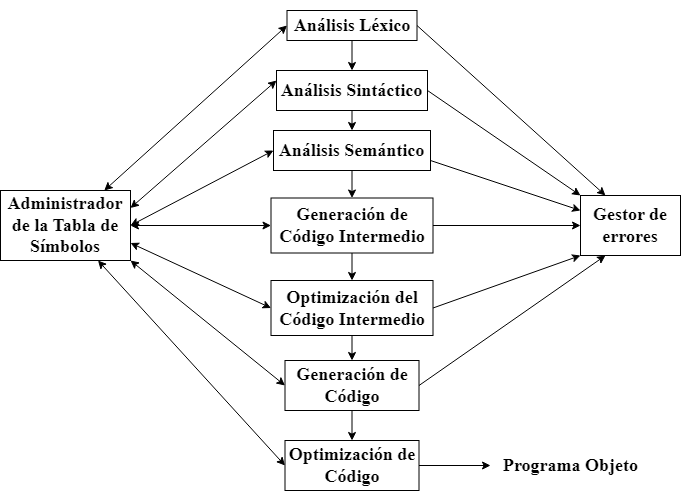
\includegraphics[scale=0.6]{figuras/Cap1/fasescomp.png} \\
    \caption{Fases Principales en el Proceso de Traducción}\label{fig:fases}
\end{figure}

\section{Definición del problema real}

Este proyecto de fin de carrera se enfoca en una tarea crucial: la corrección, mejora y ampliación de ``SimAS: Simuladores de Analizadores Sintácticos'', que es una aplicación desarrollada en java que tiene como objetivo ayudar a la docencia de la asignatura de Procesadores de Lenguajes de tercer curso de la especialidad de Computación del Grado de Ingeniería Informática. 

SimAS proporciona a los estudiantes una comprensión profunda del funcionamiento de la fase de análisis sintáctico en compiladores e intérpretes. Tiene la capacidad de simular tanto analizadores sintácticos descendentes como ascendentes, facilitando que los estudiantes comprendan mejor el funcionamiento de estos métodos de análisis sintáctico.

SimAS es una aplicación de software que posee dos versiones. SimAS 1.0 fue desarrollado por Vanesa González Pérez \cite{vanesa} como Proyecto de Fin de Carrera de Ingeniería Informática en 2015. Esta versión permitía realizar el análisis sintáctico descendente predictivo y el análisis ascendente LR (SLR, LR - canónico y LALR).  Esta versión fue corregida y ampliada en la versión SimAS 2.0, que fue desarrollada por Juan Antonio Fernández Díaz \cite{juan} en su Trabajo de Fin de Grado en 2023. Esta versión permitía generar informes en formato pdf y generar los árboles sintácticos asociados a la derivaciones de los analizadores sintácticos.


A pesar de la funcionalidad satisfactoria de SimAS, se han detectado una serie de errores y deficiencias que demandan atención inmediata.
\begin{itemize}
    \item Al cargar o modificar gramáticas, la aplicación debe ordenar sus reglas de producción en función del símbolo no terminal de la parte izquierda.
    \item Al crear o modificar gramáticas, la aplicación no genera bien el archivo XML \cite{xml} con dicha gramática.
    \item La aplicación no genera o genera de forma incorrecta los informes en formato PDF.
    \item No genera correctamente los conjuntos Primero y Siguiente de algunas gramáticas. Estos conjuntos son necesarios para realizar el análisis sintáctico descendente predictivo y el análisis sintáctico ascendente SLR.
    \item La aplicación no genera correctamente los árboles sintácticos asociados a las derivaciones.
    \item La interfaz produce algunas ventanas no interactivas o que no aportan valor.
\end{itemize}

Además, se pueden incorporar las siguientes mejoras para enriquecer la aplicación:

\begin{itemize}
    \item Diseñar una interfaz más intuitiva que genere todas las ventanas dentro de una misma interfaz y no en diferentes ventanas.
    \item Permitir el trabajo con varias gramáticas a la vez. 
    \item Implementar la posibilidad de cambiar el idioma de la aplicación.
\end{itemize}

Una descripción más detallada de las versiones de SimAS se puede consultar en el capítulo \ref{cap:antecedentes} de Antecedentes.


Aunque las versiones anteriores SimAS 1.0  y 2.0 permiten simular los análisis sintácticos descendente y ascendente, el presente Trabajo de Fin de Grado se va a centrar exclusivamente en corregir todos los fallos encontrados y en mejorar el análisis sintáctico descendente predictivo. La nueva aplicación se denominará ``SimAS 3.0 descendente predictivo''. Se considera que abordar también la corrección de los errores de la simulación del análisis sintáctico ascendente requeriría un esfuerzo superior al exigido en un Trabajo de Fin de Grado. Se debe tener en cuenta que la versión SimAS 2.0 \cite{juan} fue realizada en un Trabajo de Fin de Grado de doble especialidad que tiene una carga docente de 450 horas, superior a las 300 horas de un Trabajo de Fin de Grado de una única especialidad.


\section{Definición del problema técnico}


El presente Trabajo de Fin de Grado pretende desarrollar una aplicación informática multiplataforma, denominada ``SimAS 3.0 descendente predictivo'', que permita corregir y ampliar la simulación del análisis sintáctico descendente predictivo desarrollado en las versiones anteriores de SimAS 1.0 \cite{vanesa} y 2.0 \cite{juan}.

\subsection{Funcionamiento}
La aplicación propuesta se diseñará como una herramienta de escritorio multiplataforma con el objetivo de proporcionar a los usuarios una experiencia interactiva y educativa. Los principales módulos que integrará esta aplicación son los siguientes:

\begin{itemize}
    \item \textbf{Editor de gramáticas de contexto libre:} este módulo permitirá a los usuarios crear, cargar, guardar y modificar gramáticas de contexto libre. La interfaz proporcionará opciones intuitivas para trabajar con las reglas de producción, símbolos terminales y no terminales, así como la definición del símbolo inicial.

    \item \textbf{Simulador gráfico descendente:} esta funcionalidad simulará el proceso de análisis sintáctico descendente predictivo, utilizando la gramática especificada en el editor. El simulador generará una derivación por la izquierda y mostrará el árbol sintáctico descendente resultante.

    \item \textbf{Generación de árboles sintácticos descendentes:} se implementará la funcionalidad para generar árboles sintácticos de forma precisa y visualmente comprensible. Esta característica permitirá a los usuarios visualizar de manera clara la estructura jerárquica de las derivaciones sintácticas.
    
    \item \textbf{Tutorial interactivo:} este módulo proporcionará una guía paso a paso sobre los fundamentos y el funcionamiento de los métodos de análisis sintáctico. Los usuarios podrán acceder a explicaciones detalladas y ejemplos prácticos para comprender mejor los conceptos.
    
    \item \textbf{Ayuda integrada:} se incluirá una sección de ayuda en la interfaz para brindar asistencia instantánea sobre el uso de la aplicación. Los usuarios podrán acceder a información detallada sobre cada componente de la interfaz y los distintos módulos que componen la aplicación.
\end{itemize}

El funcionamiento detallado de cada uno de estos módulos se abordará en el capítulo \ref{cap:especificacion_requisitos} de Especificación de requisitos para proporcionar una comprensión completa de la aplicación.


\subsection{Entorno}
%Posibles modificaciones conforme se desarrolle la aplicación

El entorno en el que se desarrolla y ejecuta una aplicación es fundamental para garantizar su funcionalidad, usabilidad y despliegue efectivo. En este apartado, se detallan los aspectos relacionados con la interfaz de usuario, el entorno de desarrollo y el entorno de ejecución de la aplicación ``SimAS 3.0 descendente predictivo'', proporcionando una visión general de los componentes y requisitos clave para su funcionamiento.


\subsubsection{Interfaz con el usuario}

La aplicación contará con una interfaz gráfica de usuario (GUI\footnote{\textit{Graphical User Interface}}) diseñada para optimizar la experiencia del usuario, especialmente para los estudiantes. Se busca que todo el programa se ejecute en una única ventana, posibilitando la aparición de distintas pestañas, con el fin de simplificar la navegación. 

La interfaz estará diseñada para ser simple y completa al mismo tiempo, permitiendo a los usuarios realizar todas las operaciones necesarias para trabajar con gramáticas. Entre las funcionalidades específicas que ofrecerá la interfaz, se incluyen la capacidad de crear nuevas gramáticas e importar y editar gramáticas creadas previamente. Además, se proporcionará soporte para interacciones complejas, como la entrada de texto y la selección de archivos.

\subsubsection{Entorno de desarrollo}
El desarrollo y mantenimiento del código de la aplicación se realizará utilizando diversas fuentes de información disponibles en Internet, así como técnicas de inteligencia artificial. El entorno de desarrollo integrado (IDE) principal utilizado será IntelliJ \cite{intellij}, que ofrece una amplia gama de características y herramientas para el desarrollo de aplicaciones Java. Además, se utilizarán herramientas adicionales, como sistemas de control de versiones (Git \cite{git}) para el control del código fuente, y se gestionará la documentación y los recursos del proyecto en un repositorio de GitHub \cite{github}.

\subsubsection{Entorno de ejecución}
La aplicación estará diseñada para ser ejecutada en un entorno multiplataforma y compatible con los principales sistemas operativos, incluyendo Windows, macOS y Linux. No se requerirán configuraciones específicas del sistema operativo o del entorno de ejecución para garantizar el funcionamiento correcto de la aplicación. Además, la aplicación se ejecutará en una máquina virtual de Java \cite{java}, lo que proporcionará una mayor portabilidad y compatibilidad con diferentes sistemas. Esto significa que los usuarios finales no necesitarán instalar ninguna dependencia externa ni cumplir con requisitos adicionales de instalación, lo que facilitará su despliegue y uso.


\subsection{Ciclo de mantenimiento} \label{subsec:actualizaciones}

La gestión de actualizaciones de software es un proceso crítico que garantiza la evolución continua y la mejora de la aplicación a lo largo del tiempo. En el caso de ``SimAS 3.0 descendente predictivo'', se implementará un ciclo de mantenimiento diseñado para abordar nuevas funcionalidades, correcciones de errores y adaptaciones a los cambios en los entornos de ejecución.

El ciclo de mantenimiento de ``SimAS 3.0 descendente predictivo'' se basará en un enfoque proactivo y modular, permitiendo la incorporación de mejoras de manera eficiente y sin interrupciones significativas en la experiencia del usuario. Aunque el autor principal del proyecto no asumirá la responsabilidad directa del mantenimiento futuro, se establecerán procedimientos claros para la gestión de actualizaciones, asegurando la continuidad y la calidad del software.

Este enfoque modular no solo facilitará el mantenimiento y la actualización del software, sino que también fomentará la colaboración y la contribución de la comunidad de usuarios y desarrolladores. De esta manera, SimAS 3.0 podrá adaptarse de manera ágil a las necesidades cambiantes de los usuarios y a las demandas del entorno tecnológico.


\subsection{Competencia}

El desarrollo de SimAS 3.0 se sitúa en un contexto de continua evolución y expansión en el ámbito de las herramientas educativas para el análisis sintáctico en la informática. Aunque no buscamos competir comercialmente, es importante comprender el panorama actual y las características distintivas de SimAS 3.0 en relación con otras soluciones disponibles.

A través de un análisis exhaustivo en el Capítulo \ref{cap:antecedentes}, se explorará el terreno de las herramientas educativas existentes para el análisis sintáctico. Se examinarán tanto las aplicaciones desarrolladas en proyectos académicos previos, como otras soluciones disponibles en el mercado. Este análisis permitirá identificar fortalezas, debilidades y oportunidades de mejora para SimAS 3.0.

Si bien se reconocen las contribuciones de otras herramientas educativas, SimAS 3.0 buscará destacarse por su enfoque innovador y sus funcionalidades distintivas. Entre estas funcionalidades, se encuentra la capacidad de generar árboles sintácticos tanto descendentes como ascendentes, ofreciendo una experiencia de aprendizaje única y completa para los estudiantes de informática.


%Posibles modificaciones durante el desarrollo
\subsection{Aspecto externo}

En esta sección, se abordarán aspectos clave relacionados con la experiencia del usuario y la documentación asociada a SimAS 3.0.

\begin{itemize}
    \item \textbf{Diseño de la interfaz de usuario}: la interfaz de usuario de SimAS 3.0 se diseñará cuidadosamente para garantizar una experiencia visual atractiva y una navegación intuitiva. Se prestará especial atención a la disposición de los elementos, la coherencia visual y la accesibilidad, con el objetivo de proporcionar un entorno de trabajo cómodo y eficiente para los usuarios.
    
    \item \textbf{Documentación detallada}:
    \begin{itemize}
        \item \textit{Manual técnico}: este documento proporcionará una descripción exhaustiva de los aspectos técnicos del desarrollo de SimAS 3.0. Se incluirán detalles sobre la arquitectura del software, las tecnologías utilizadas y las decisiones de diseño fundamentales.
        
        \item \textit{Manual de usuario}: el manual de usuario de SimAS 3.0 contendrá instrucciones claras y concisas sobre la instalación, configuración y uso de la aplicación. Se incluirán ejemplos prácticos y capturas de pantalla para guiar al usuario a través de las diferentes funcionalidades de la aplicación.
        
        \item \textit{Manual de código}: este documento estará dirigido a desarrolladores y proporcionará una visión detallada del código fuente de SimAS 3.0. Se describirá la estructura del proyecto, las convenciones de codificación y la documentación interna del código para facilitar su comprensión y mantenimiento.
    \end{itemize}
    
    \item \textbf{Distribución y almacenamiento}: SimAS 3.0 estará disponible para su descarga en línea a través de un repositorio público, lo que facilitará el acceso a la última versión del software y de la documentación asociada. Además, se explorarán opciones para distribuir la aplicación en medios físicos o mediante servicios de almacenamiento en la nube, asegurando así su disponibilidad y accesibilidad para los usuarios.
\end{itemize}


\subsection{Estandarización}

En esta sección, se describirán los principios de diseño y usabilidad que guiarán el desarrollo de SimAS 3.0, con el objetivo de garantizar una experiencia de usuario coherente y satisfactoria.

\begin{itemize}
    \item \textbf{Diseño centrado en el usuario}: SimAS 3.0 se diseñará pensando en las necesidades y expectativas del usuario final. Se realizarán investigaciones de usuarios y pruebas de usabilidad para asegurar que la interfaz de usuario sea intuitiva y fácil de usar.
    
    \item \textbf{Consistencia y coherencia}: la interfaz de usuario de SimAS 3.0 mantendrá una apariencia y comportamiento coherentes en todas sus funciones y elementos. Se seguirán estándares de diseño reconocidos y se aplicarán patrones de diseño comunes para garantizar una experiencia consistente para el usuario.
    
    \item \textbf{Sensibilidad y guía del usuario}: la interfaz de SimAS 3.0 guiará al usuario a través de la aplicación, proporcionando retroalimentación clara y orientación en cada paso del proceso. Se utilizarán mensajes informativos y visuales para informar al usuario sobre el estado y las acciones disponibles.
    
    \item \textbf{Interacción intuitiva}: se priorizará una interacción sencilla y fluida en SimAS 3.0. Los controles y las funciones de la aplicación se diseñarán de manera intuitiva, minimizando la necesidad de aprendizaje por parte del usuario y facilitando el uso de la aplicación desde el primer momento.
    
    \item \textbf{Claridad y legibilidad}: la interfaz gráfica de SimAS 3.0 se diseñará con un enfoque en la claridad y la legibilidad. Se utilizarán colores y tipografías adecuados para garantizar una fácil comprensión de la información presentada, evitando la sobrecarga visual y la confusión del usuario.
\end{itemize}


\subsection{Calidad y fiabilidad}

En esta sección, se abordarán los aspectos de calidad, fiabilidad y seguridad que son fundamentales en el desarrollo y uso de SimAS 3.0. Se buscará garantizar el correcto funcionamiento de la aplicación, así como proteger la integridad y privacidad de los usuarios.

\begin{itemize}
    \item \textbf{Calidad y fiabilidad}: SimAS 3.0 se desarrollará con un enfoque en la calidad del software y la fiabilidad de su funcionamiento. Se utilizarán herramientas actualizadas como IntelliJ IDEA y la Máquina Virtual de Java para respaldar la calidad del código y su ejecución. Además, la aplicación será sometida a exhaustivas pruebas para detectar y corregir errores antes de su lanzamiento.
    
    \item \textbf{Seguridad}: la seguridad de SimAS 3.0 será una prioridad, tanto en términos de protección contra acciones incorrectas por parte del usuario como en la seguridad del dispositivo de almacenamiento. Se implementarán mecanismos de seguridad en la aplicación para evitar cualquier manipulación maliciosa o acceso no autorizado a los datos del usuario. Se garantizará que el usuario no tenga acceso a ninguna funcionalidad aparte de aquellas proporcionadas explícitamente por la aplicación, asegurando así que no se realicen acciones no deseadas ni se acceda a datos sensibles. Asimismo, se garantizará que la distribución y uso de la aplicación cumplan con los principios de software libre, siguiendo la licencia GPL de GNU para proteger su distribución y uso adecuados.
\end{itemize}


\subsection{Validación y verificación}

El proceso de validación y verificación de SimAS 3.0 es esencial para garantizar su correcto funcionamiento y la detección temprana de posibles errores.

\begin{itemize}
    \item \textbf{Validación}: se centrará en asegurar que la aplicación cumple con los requisitos y expectativas del usuario final. Se llevarán a cabo pruebas funcionales para verificar que todas las funcionalidades operan según lo esperado, y se realizarán pruebas de aceptación para garantizar que la aplicación satisface las necesidades del usuario.
    
    \item \textbf{Verificación}: por otro lado, se centrará en asegurar que el código y la lógica de la aplicación son correctos y libres de errores. Se realizarán pruebas unitarias para verificar el correcto funcionamiento de cada componente individualmente, así como pruebas de integración para garantizar que los componentes interactúan correctamente entre sí.
\end{itemize}

El proceso estará dividido en varias etapas, cada una con su respectiva documentación detallada:

\begin{itemize}
    \item \textbf{Planificación de pruebas}: se definirán los objetivos y alcance de las pruebas, así como los recursos y herramientas necesarios para llevarlas a cabo.
    
    \item \textbf{Diseño de pruebas}: se elaborará un plan detallado de las pruebas a realizar, incluyendo los casos de prueba específicos y los criterios de aceptación.
    
    \item \textbf{Ejecución de pruebas}: se llevarán a cabo las pruebas según el plan establecido, registrando los resultados obtenidos y cualquier incidencia detectada.
    
    \item \textbf{Análisis de resultados}: se analizarán los resultados de las pruebas para identificar posibles áreas de mejora o corrección. Se documentarán los errores encontrados y se propondrán soluciones para su resolución.
\end{itemize}

El capítulo \ref{cap:pruebas} detallará cada una de estas etapas y proporcionará una visión completa del proceso de validación y verificación de SimAS 3.0.


\subsection{Programa de tareas}

El desarrollo del Trabajo de Fin de Grado estará compuesto por las siguientes actividades:
\begin{enumerate}
    \item \textbf{Exploración inicial} 
        \begin{itemize}
            \item Comprensión y prueba de SimAS 2.0 \cite{juan}.
            \item Definición del problema técnico.
            \item Establecimiento de los objetivos.
            \item Revisión de los antecedentes.
            \item Identificación de los recursos iniciales y estratégicos.
            \item Selección de las herramientas de software y hardware.
            \item Investigación del entorno Intellij \cite{intellij} y del lenguaje de programación Java \cite{java}.
        \end{itemize}
    \item \textbf{Análisis y diseño}
        \begin{itemize}
            \item Especificación de requisitos: funcionales, no funcionales, de información y de la interfaz.
            \item Elaboración de los casos de uso.
            \item Validación de los casos de uso.
            \item Elaboración de los diagramas de secuencia.
        \end{itemize}
    \item \textbf{Diseño}
        \begin{itemize}
            \item Diseño de la arquitectura del sistema.
            \item Diseño de paquetes y clases.
            \item Diseño de la interfaz
        \end{itemize}        
    \item \textbf{Implementación}
        \begin{itemize}
            \item Desarrollo del código.
            \item Implementación de pruebas unitarias.
            \item Validación del código desarrollado.
        \end{itemize} 
    \item \textbf{Documentación}
      \begin{itemize}
          \item Elaboración del manual técnico, manual de usuario y manual de código.
          \item La redacción del manual técnico se realizará durante todo el proceso de desarrollo del Trabajo de Fin de Grado.
      \end{itemize}
\end{enumerate}

\subsection{Pruebas}
Las pruebas y la validación son elementos esenciales en el desarrollo de cualquier aplicación. Estos procesos permiten asegurar que la aplicación cumpla con los estándares de calidad y funcionalidad esperados. En el caso de SimAS 3.0, se llevarán a cabo diversas actividades de evaluación y validación para garantizar su correcto funcionamiento y fiabilidad.

\subsubsection{Tipos de Pruebas}

Se llevarán a cabo varios tipos de pruebas para evaluar distintos aspectos de SimAS 3.0:

\begin{itemize}
    \item \textbf{Pruebas de Funcionalidad:} estas pruebas se centran en verificar que todas las funciones y características de SimAS 3.0 funcionen como se espera. Se realizarán pruebas exhaustivas para cada módulo y componente de la aplicación.
    
    \item \textbf{Pruebas de Interfaz de Usuario:} estas pruebas se enfocarán en la usabilidad y la experiencia del usuario. Se evaluará la interfaz gráfica para garantizar que sea intuitiva y fácil de usar.

    \item \textbf{Pruebas de Rendimiento:} se llevarán a cabo pruebas para evaluar el rendimiento y la velocidad de SimAS 3.0, especialmente en situaciones de carga y con grandes conjuntos de datos.

    \item \textbf{Pruebas de Compatibilidad:} se realizarán pruebas en diferentes sistemas operativos y entornos de ejecución para garantizar que SimAS 3.0 funcione correctamente en diversas configuraciones.
\end{itemize}

\subsubsection{Descripción de las Pruebas}

Cada prueba estará estructurada de la siguiente manera:

\begin{itemize}
    \item \textbf{Objetivo:} se definirá claramente el objetivo de la prueba, es decir, qué se espera evaluar o validar.
    
    \item \textbf{Problema:} se identificarán y documentarán los problemas o errores detectados durante la ejecución de la prueba, junto con información detallada sobre cómo reproducirlos.

    \item \textbf{Solución:} se propondrán soluciones y acciones correctivas para abordar los problemas identificados durante las pruebas, asegurando así la mejora continua de la aplicación.
\end{itemize}

El próximo capítulo \ref{cap:pruebas} detallará los procedimientos y resultados de las pruebas llevadas a cabo en ``SimAS 3.0 descendente predictivo'' como parte de este Trabajo de Fin de Grado.


\subsection{Seguridad}
La seguridad en la presente aplicación se centra principalmente en garantizar su correcto funcionamiento sin comprometer la integridad de los sistemas donde se ejecute. Dado que la aplicación no maneja ni almacena datos personales de los usuarios, el enfoque de seguridad se orienta hacia la prevención de posibles daños a los equipos o entornos de ejecución.

Se implementarán medidas para asegurar que durante la ejecución de la aplicación, los usuarios no puedan realizar acciones que puedan comprometer su funcionamiento o la estabilidad del sistema. Además, se prestará especial atención a la protección del dispositivo de almacenamiento donde se ejecute la aplicación, garantizando que no se produzcan daños o alteraciones no deseadas.

En línea con la versión anterior, la aplicación se distribuirá libremente, sin restricciones de uso, copia o distribución. Esto se fundamenta en su naturaleza académica y en su carácter no lucrativo. No se aplicarán medidas de protección contra la distribución libre de la aplicación, permitiendo su acceso y uso por parte de cualquier usuario interesado en aprender o utilizarla con fines educativos.

En cuanto a la licencia, la aplicación seguirá los principios de la Licencia Pública General de GNU (GPL), que garantiza la libertad de uso, modificación y redistribución del software. Esta licencia ayuda a prevenir acciones malintencionadas relacionadas con la copia o reproducción del software, asegurando que permanezca accesible para la comunidad académica y de desarrollo de software.
\part{Documentación externa}
\chapter{Recursos y Requisitos de desarrollo y ejecución}\label{cap-requisitos-desarrollo-ejecucion}

\section{Introducción}


\section{Recursos}
	

\section{Recursos de hardware}

\section{Recursos de software}


	
\section{Entorno de Desarrollo}



\section{Descripción modular}


\part{Documentación interna}
\chapter{Código de la aplicación}\label{cap-documentacion-interna}


\section{Ejemplo USANDO MINTED}

\inputminted[linenos,breaklines]{java}{codigo/SimAs/Bienvenida.java}


\section{Ejemplo USANDO lstinputlisting}
	
%\lstinputlisting[language=Java]{doc/name.tex}
 
\section{Paquete SimAS}	

\subsection{Bienvenida.java}

\lstinputlisting[language=Java,breaklines=true]{codigo/SimAs/Bienvenida.java}


\chapter{Documentación de Paquetes}\label{cap-documentacion-paquetes}

\section{Introducción}

Este capítulo proporciona una documentación detallada de cada paquete Java que constituye la aplicación SimAS 3.0. Para cada paquete se incluye una descripción de su propósito, las clases que contiene, las relaciones con otros paquetes y referencias directas al código fuente en el repositorio.

\textbf{Referencias al Manual Técnico:} Para explicaciones más detalladas sobre la arquitectura de paquetes, diagramas de dependencias completos, métricas de complejidad, análisis de acoplamiento/cohesión y patrones de diseño implementados, consulte:
\begin{itemize}
    \item Capítulo 8: "Diseño de paquetes" - Arquitectura completa y análisis detallado de dependencias.
    \item Capítulo 9: "Diseño de clases" - Implementación detallada de todas las clases del sistema.
\end{itemize}

La arquitectura de paquetes sigue principios de diseño orientado a objetos con separación clara de responsabilidades, bajo acoplamiento y alta cohesión. El sistema está organizado en 8 paquetes principales distribuidos en capas funcionales.

\section{Arquitectura general de paquetes}

SimAS 3.0 está estructurado siguiendo una \textit{arquitectura modular por capas} con separación clara de responsabilidades:

\begin{itemize}
    \item \textbf{Capa de Presentación} (\texttt{bienvenida, vistas}): gestiona la interfaz de usuario.
    \item \textbf{Capa de Lógica de Negocio} (\texttt{editor, simulador}): implementa la funcionalidad principal.
    \item \textbf{Capa de Modelo de Datos} (\texttt{gramatica}): representa las estructuras de datos fundamentales
    \item \textbf{Capa de Servicios Transversales} (\texttt{utils}): proporciona funcionalidades comunes.
    \item \textbf{Capa de Recursos} (\texttt{resources}): contiene recursos estáticos.
    \item \textbf{Capa de Documentación} (\texttt{centroayuda}): proporciona ayuda y documentación.
\end{itemize}

\textbf{Referencia a la arquitectura completa:} Consulte el Capítulo 8 del Manual Técnico para análisis detallado de la arquitectura de paquetes.

\section{Paquete bienvenida}

\subsection{Propósito}

El paquete \texttt{bienvenida} implementa la \textit{capa de presentación inicial} del sistema, actuando como punto de entrada principal de SimAS 3.0. Este paquete es fundamental para la experiencia del usuario, proporcionando una interfaz intuitiva y profesional.

\textbf{Ubicación en el repositorio:} \url{https://github.com/Llamatekee/SimAS-3.0/tree/main/src/bienvenida}

\textbf{Responsabilidades principales:}
\begin{itemize}
    \item Gestión completa del ciclo de vida inicial de la aplicación.
    \item Navegación centralizada hacia módulos funcionales.
    \item Coordinación entre componentes de la interfaz principal.
    \item Gestión de estados globales de la aplicación.
\end{itemize}

\subsection{Clases principales}

\subsubsection{Clase Bienvenida}

Clase principal que gestiona la pantalla de bienvenida de la aplicación.

\textbf{Ubicación:} \url{https://github.com/Llamatekee/SimAS-3.0/blob/main/src/bienvenida/Bienvenida.java}

\begin{itemize}
    \item \textbf{Herencia}: Extiende \texttt{Application} de JavaFX.
    \item \textbf{Patrón implementado}: Singleton para garantizar instancia única.
    \item \textbf{Responsabilidades}:
    \begin{itemize}
        \item Mostrar la pantalla de bienvenida con información del proyecto.
        \item Gestionar la transición automática al menú principal (2.5 segundos).
        \item Configurar el estilo y comportamiento de la ventana de bienvenida.
        \item Soporte completo de internacionalización.
    \end{itemize}
    \item \textbf{Métodos principales}:
    \begin{itemize}
        \item \texttt{start(Stage)}: inicializa la ventana de bienvenida
        \item \texttt{abrirMenuPrincipal()}: transita al menú principal
        \item \texttt{main(String[])}: punto de entrada estático
    \end{itemize}
\end{itemize}

\subsubsection{Clase MenuPrincipal}

Controlador principal que gestiona el menú principal de la aplicación y coordina la navegación.

\textbf{Ubicación:} \url{https://github.com/Llamatekee/SimAS-3.0/blob/main/src/bienvenida/MenuPrincipal.java}

\begin{itemize}
    \item \textbf{Herencia}: extiende \texttt{Application} de JavaFX.
    \item \textbf{Patrón implementado}: Facade para simplificar acceso a módulos complejos.
    \item \textbf{Responsabilidades}:
    \begin{itemize}
        \item Gestionar la interfaz del menú principal con sistema de pestañas avanzado.
        \item Coordinar la apertura de diferentes módulos (editor, simulador, ayuda).
        \item Implementar internacionalización completa con cambio dinámico de idioma.
        \item Gestionar sistema de ventanas secundarias y arrastrar/soltar pestañas.
        \item Configurar atajos de teclado para operaciones frecuentes.
        \item Gestionar navegación contextual y estados de la aplicación.
    \end{itemize}
    \item \textbf{Métodos principales}:
    \begin{itemize}
        \item \texttt{start(Stage)}: inicializa la ventana principal completa.
        \item \texttt{cambiarIdioma()}: gestiona cambio dinámico de idioma.
        \item \texttt{onBtnEditorAction()}: abre nueva instancia del editor.
        \item \texttt{onBtnSimuladorAction()}: carga gramática y abre simulador.
        \item \texttt{onBtnAyudaAction()}: abre documentación en navegador.
    \end{itemize}
\end{itemize}

\subsection{Dependencias y relaciones}

\begin{itemize}
    \item \textbf{Dependencias críticas}:
    \begin{itemize}
        \item \texttt{utils.*}: sistema de internacionalización, gestión de pestañas y ventanas (\textbf{85\% del sistema}).
        \item \texttt{resources}: iconos y recursos gráficos para la interfaz.
        \item \texttt{vistas}: archivos FXML para definición de interfaces.
    \end{itemize}
    \item \textbf{Relaciones con otros paquetes}:
    \begin{itemize}
        \item \texttt{editor}: crea instancias del editor de gramáticas.
        \item \texttt{simulador}: coordina lanzamiento del simulador descendente.
        \item \texttt{centroayuda}: integra sistema de ayuda contextual.
        \item \texttt{gramatica}: utiliza modelo de datos para gestión de gramáticas.
    \end{itemize}
\end{itemize}

\textbf{Características técnicas:}
\begin{itemize}
    \item \textbf{Complejidad}: 2 clases (5\% del total del sistema).
    \item \textbf{Patrones implementados}: Singleton, Facade, MVC (Vista-Controlador).
    \item \textbf{Responsabilidad}: punto de entrada único y navegación centralizada.
\end{itemize}

\section{Paquete editor}

\subsection{Propósito}

El paquete \texttt{editor} implementa el \textit{núcleo funcional de edición de gramáticas} de SimAS 3.0, proporcionando una interfaz completa para la creación, modificación y gestión de gramáticas de contexto libre. Este paquete representa el componente más complejo del sistema, con 10 clases que implementan un asistente paso a paso altamente sofisticado.

\textbf{Ubicación en el repositorio:} \url{https://github.com/Llamatekee/SimAS-3.0/tree/main/src/editor}

\textbf{Arquitectura y diseño:}

El paquete sigue una \textit{arquitectura modular jerárquica} organizada en tres niveles:
\begin{enumerate}
    \item \textbf{Nivel de Control Principal}: \texttt{Editor} y \texttt{EditorWindow} (gestión global).
    \item \textbf{Nivel de Coordinación}: \texttt{PanelCreacionGramatica} (orquestación del asistente).
    \item \textbf{Nivel de Especialización}: paneles específicos por funcionalidad.
\end{enumerate}

\subsection{Clases principales}

\subsubsection{Clase Editor}

Clase principal del editor que coordina todos los paneles de edición y gestiona el estado global.

\textbf{Ubicación:} \url{https://github.com/Llamatekee/SimAS-3.0/blob/main/src/editor/Editor.java}

\begin{itemize}
    \item \textbf{Herencia}: extiende \texttt{VBox} de JavaFX e implementa \texttt{ActualizableTextos}
    \item \textbf{Patrón implementado}: Mediator para coordinar comunicación entre paneles.
    \item \textbf{Responsabilidades}:
    \begin{itemize}
        \item Gestionar la gramática activa y su estado.
        \item Coordinar todos los paneles del asistente de creación.
        \item Implementar patrón Mediator para comunicación entre componentes.
        \item Gestionar persistencia de datos y validación global.
        \item Coordinar navegación entre pasos del asistente.
        \item Gestionar integración con el sistema de pestañas.
    \end{itemize}
    \item \textbf{Métodos principales}:
    \begin{itemize}
        \item \texttt{Editor(TabPane, MenuPrincipal)}: constructor con configuración completa.
        \item \texttt{cargarGramatica(Gramatica)}: carga gramática para edición.
        \item \texttt{validarGramaticaActual()}: validación completa de la gramática.
        \item \texttt{guardarGramatica()}: persistencia de datos.
    \end{itemize}
\end{itemize}

\subsubsection{EditorWindow.java}

Ventana principal del editor que contiene todos los paneles de edición.

\begin{itemize}
    \item \textbf{Responsabilidades}:
    \begin{itemize}
        \item Gestionar la interfaz de usuario del editor.
        \item Coordinar la navegación entre paneles.
        \item Gestionar el estado de la gramática en edición.
    \end{itemize}
\end{itemize}

\subsubsection{PanelCreacionGramatica.java}

Panel base que define la estructura común para todos los paneles de creación.

\subsubsection{PanelCreacionGramaticaPaso1.java}

Panel para la definición del nombre y descripción de la gramática.

\subsubsection{PanelCreacionGramaticaPaso2.java}

Panel para la definición de símbolos terminales y no terminales de la gramática.

\subsubsection{PanelCreacionGramaticaPaso3.java}

Panel para la definición de producciones de la gramática.

\subsubsection{PanelCreacionGramaticaPaso4.java}

Panel para la definición del símbolo inicial y validación de la gramática.

\subsubsection{PanelProducciones.java}

Panel especializado para la gestión de producciones con funcionalidades avanzadas.

\subsubsection{PanelSimbolosNoTerminales.java}

Panel especializado para la gestión de símbolos no terminales.

\subsubsection{PanelSimbolosTerminales.java}

Panel especializado para la gestión de símbolos terminales.

\subsection{Dependencias}

\begin{itemize}
    \item \texttt{gramatica.*}: para el modelo de datos de gramáticas.
    \item \texttt{utils.*}: para utilidades de interfaz y gestión de ventanas.
    \item \texttt{vistas.*}: para las definiciones FXML de la interfaz.
\end{itemize}

\section{Paquete gramatica}

\subsection{Propósito}

El paquete \texttt{gramatica} contiene el modelo de datos y los algoritmos fundamentales para el manejo de gramáticas libres de contexto y la generación de tablas de análisis predictivo.

\subsection{Clases principales}

\subsubsection{Gramatica.java}

Clase central que representa una gramática libre de contexto completa.

\begin{itemize}
    \item \textbf{Responsabilidades}:
    \begin{itemize}
        \item Almacenar todos los componentes de una gramática.
        \item Implementar algoritmos de análisis sintáctico.
        \item Generar tablas de análisis predictivo.
        \item Validar la gramática y detectar conflictos.
    \end{itemize}
    \item \textbf{Métodos principales}:
    \begin{itemize}
        \item \texttt{generarTablaPredictiva()}: genera la tabla de análisis predictivo.
        \item \texttt{calcularFirst()}: calcula los conjuntos PRIMERO.
        \item \texttt{calcularFollow()}: calcula los conjuntos SIGUIENTE.
        \item \texttt{esLL1()}: verifica si la gramática es LL(1).
    \end{itemize}
\end{itemize}

\subsubsection{Simbolo.java}

Clase abstracta base para todos los símbolos de la gramática.

\subsubsection{Terminal.java}

Representa un símbolo terminal de la gramática.

\subsubsection{NoTerminal.java}

Representa un símbolo no terminal de la gramática.

\subsubsection{Produccion.java}

Representa una producción de la gramática con su antecedente y consecuente.

\subsubsection{Antecedente.java}

Representa el lado izquierdo de una producción (no terminal).

\subsubsection{Consecuente.java}

Representa el lado derecho de una producción (secuencia de símbolos).

\subsubsection{TablaPredictiva.java}

Clase base para la representación de tablas de análisis predictivo.

\subsubsection{TablaPredictivaPaso5.java}

Implementación específica de la tabla predictiva con funcionalidades avanzadas.

\subsubsection{FilaTablaPredictiva.java}

Representa una fila de la tabla predictiva.

\subsubsection{FuncionError.java}

Representa una función de error personalizada para el análisis.

\subsection{Algoritmos implementados}

\subsubsection{Cálculo de conjuntos PRIMERO}

El algoritmo calcula para cada símbolo no terminal el conjunto de símbolos terminales que pueden aparecer al inicio de las cadenas derivadas.

\subsubsection{Cálculo de conjuntos SIGUIENTE}

El algoritmo calcula para cada símbolo no terminal el conjunto de símbolos terminales que pueden aparecer inmediatamente después de él en alguna derivación.

\subsubsection{Generación de tabla predictiva}

Utiliza los conjuntos PRIMERO y SIGUIENTE para construir la tabla de análisis predictivo LL(1).

\subsection{Dependencias}

Este paquete es independiente y no tiene dependencias externas, sirviendo como base para otros paquetes.

\section{Paquete simulador}

\subsection{Propósito}

El paquete \texttt{simulador} implementa el simulador de análisis sintáctico descendente predictivo, permitiendo a los usuarios simular el proceso de análisis paso a paso.

\subsection{Clases principales}

\subsubsection{PanelSimuladorDesc.java}

Panel principal del simulador que coordina todos los componentes de simulación.

\subsubsection{PanelSimulacion.java}

Panel que gestiona la interfaz de usuario del simulador y el estado de la simulación.

\subsubsection{SimulacionFinal.java}

Clase que implementa la lógica de simulación del análisis sintáctico.

\subsubsection{PanelNuevaSimDescPaso*.java}

Conjunto de paneles para la configuración paso a paso de una nueva simulación.

\subsubsection{EditorCadenaEntradaController.java}

Controlador para la edición de cadenas de entrada a analizar.

\subsubsection{NuevaFuncionError.java}

Panel para la creación de nuevas funciones de error personalizadas.

\subsubsection{PanelGramaticaOriginal.java}

Panel que muestra la gramática original utilizada en la simulación.

\subsection{Características del simulador}

\begin{itemize}
    \item Simulación paso a paso del análisis sintáctico.
    \item Visualización de la pila de análisis.
    \item Visualización del estado de la entrada.
    \item Generación del árbol de derivación.
    \item Manejo de errores con funciones personalizadas.
    \item Interfaz intuitiva con controles de navegación.
\end{itemize}

\subsection{Dependencias}

\begin{itemize}
    \item \texttt{gramatica.*}: para acceso a gramáticas y tablas predictivas.
    \item \texttt{utils.*}: para utilidades de interfaz.
    \item \texttt{vistas.*}: para las definiciones FXML.
\end{itemize}

\section{Paquete utils}

\subsection{Propósito}

El paquete \texttt{utils} contiene utilidades generales, servicios de internacionalización y herramientas de gestión de ventanas que son utilizadas por toda la aplicación.

\subsection{Clases principales}

\subsubsection{SecondaryWindow.java}

Utilidad para la gestión de ventanas secundarias de la aplicación.

\subsubsection{TabManager.java}

Gestiona el sistema de pestañas para múltiples proyectos simultáneos.

\subsubsection{TabPaneMonitor.java}

Monitor que gestiona el estado y comportamiento de las pestañas.

\subsubsection{ActualizableTextos.java}

Interfaz para componentes que pueden actualizar sus textos según el idioma seleccionado.

\subsubsection{LanguageItem.java}

Representa un elemento de idioma en el sistema de internacionalización.

\subsubsection{LanguageListCell.java}

Celda personalizada para la visualización de idiomas en listas.

\subsection{Sistema de internacionalización}

El paquete incluye archivos de propiedades para múltiples idiomas:

\begin{itemize}
    \item \verb|messages_es.properties|: textos en español.
    \item \verb|messages_en.properties|: textos en inglés.
    \item \verb|messages_de.properties|: textos en alemán.
    \item \verb|messages_fr.properties|: textos en francés.
    \item \verb|messages_ja.properties|: textos en japonés.
    \item \verb|messages_pt.properties|: textos en portugués.
\end{itemize}

\subsection{Dependencias}

Este paquete es independiente y proporciona servicios a otros paquetes.

\section{Paquete centroayuda}

\subsection{Propósito}

El paquete \texttt{centroayuda} implementa el sistema de ayuda integrado de la aplicación, incluyendo documentación, tutoriales y información sobre el proyecto.

\subsection{Clases principales}

\subsubsection{AcercaDe.java}

Ventana que muestra información sobre la aplicación, desarrolladores y versión.

\subsection{Recursos incluidos}

\begin{itemize}
    \item \texttt{ayuda.html}: documentación principal de ayuda.
    \item \texttt{SimAS.html}: información específica sobre la aplicación.
    \item \verb|Tema_*.pdf|: documentos temáticos sobre análisis sintáctico.
    \item \texttt{imagenes/}: recursos gráficos para la documentación.
\end{itemize}

\subsection{Dependencias}

\begin{itemize}
    \item \texttt{utils.*}: para utilidades de interfaz.
\end{itemize}

\section{Paquete vistas}

\subsection{Propósito}

El paquete \texttt{vistas} contiene todos los archivos FXML que definen las interfaces de usuario de la aplicación, siguiendo el patrón de separación de vista y lógica.

\subsection{Archivos FXML principales}

\begin{itemize}
    \item \texttt{Bienvenida.fxml}: pantalla de bienvenida.
    \item \texttt{MenuPrincipal.fxml}: menú principal de la aplicación.
    \item \texttt{Editor.fxml}: interfaz principal del editor.
    \item \texttt{PanelCreacionGramaticaPaso*.fxml}: paneles de creación de gramáticas.
    \item \texttt{PanelSimulacion.fxml}: interfaz del simulador.
    \item \texttt{SimulacionFinal.fxml}: interfaz de simulación final.
    \item \texttt{styles2.css}: estilos CSS para la aplicación.
\end{itemize}

\subsection{Características de las vistas}

\begin{itemize}
    \item Diseño responsivo y adaptable.
    \item Uso de estilos CSS para personalización.
    \item Integración con el sistema de internacionalización.
    \item Separación clara entre presentación y lógica.
\end{itemize}

\section{Métricas y análisis de la arquitectura}

\subsection{Distribución de clases por paquete}

Con el conocimiento detallado de las 39 clases documentadas, podemos proporcionar métricas precisas sobre la complejidad del sistema:

\begin{table}[H]
\centering
\caption{Distribución de clases Java por paquete}
\label{tab:distribucion-clases}
\begin{tabular}{|l|c|c|}
\hline
\textbf{Paquete} & \textbf{Número de clases} & \textbf{Porcentaje} \\
\hline
simulador & 13 & 33\% \\
editor & 10 & 26\% \\
gramatica & 8 & 21\% \\
utils & 6 & 15\% \\
bienvenida & 2 & 5\% \\
\hline
\textbf{Total} & \textbf{39} & \textbf{100\%} \\
\hline
\end{tabular}
\end{table}

\subsection{Matriz de dependencias completa}

\begin{table}[H]
\centering
\caption{Matriz de dependencias entre paquetes}
\label{tab:matriz-dependencias}
\begin{tabular}{|l|c|c|c|c|c|c|c|c|}
\hline
\textbf{De $\rightarrow$ A} & bienv. & editor & sim. & gram. & utils & res. & centro & vistas \\
\hline
\hline
bienvenida & - & → & → & - & → & → & - & → \\
editor & - & - & - & → & → & → & → & → \\
simulador & - & - & - & → & → & → & → & → \\
gramatica & - & - & - & - & - & - & - & - \\
utils & - & - & - & - & - & - & - & - \\
resources & - & - & - & - & - & - & - & - \\
centroayuda & - & - & - & - & - & → & - & - \\
vistas & - & - & - & - & - & - & - & - \\
\hline
\end{tabular}
\end{table}

\subsection{Complejidad algorítmica por paquete}

\begin{table}[H]
\centering
\caption{Complejidad algorítmica de los paquetes principales}
\label{tab:complejidad-paquetes}
\begin{tabular}{|l|l|}
\hline
\textbf{Paquete} & \textbf{Complejidad algorítmica} \\
\hline
gramatica & O(n) a O(n³) (cálculo de conjuntos, construcción de tabla) \\
simulador & O(n³) (algoritmos de análisis sintáctico) \\
editor & O(n²) (validación y transformación de gramáticas) \\
utils & O(1) a O(n) (gestión de componentes y navegación) \\
bienvenida & O(1) (navegación básica) \\
\hline
\end{tabular}
\end{table}

\subsection{Análisis de acoplamiento y cohesión}

\begin{itemize}
    \item \textbf{Acoplamiento bajo}: las dependencias están claramente definidas y minimizadas.
    \item \textbf{Cohesión alta}: las clases dentro de cada paquete comparten fuerte relación funcional.
    \item \textbf{Punto único de fallo}: el paquete \texttt{gramatica} es crítico para todo el sistema.
    \item \textbf{Servicios transversales}: los paquetes \texttt{utils} y \texttt{resources} son utilizados por el 85\% del sistema.
\end{itemize}

\textbf{Referencias al repositorio:}

\begin{itemize}
    \item \textbf{Código fuente completo}: \url{https://github.com/Llamatekee/SimAS-3.0/tree/main/src}
    \item \textbf{Recursos del sistema}: \url{https://github.com/Llamatekee/SimAS-3.0/tree/main/src/resources}
    \item \textbf{Archivos de interfaz}: \url{https://github.com/Llamatekee/SimAS-3.0/tree/main/src/vistas}
    \item \textbf{Documentación técnica}: consulte Capítulo 8 del Manual Técnico para análisis detallado.
\end{itemize}

\chapter{Sistema de Internacionalización}\label{cap-internacionalizacion}

\section{Introducción}

SimAS 3.0 implementa un sistema completo de internacionalización (i18n) que permite a la aplicación adaptarse a diferentes idiomas y regiones. Este sistema soporta 6 idiomas completos con conmutación en tiempo de ejecución, facilitando el acceso a usuarios de diferentes países y culturas.

\textbf{Ubicación en el repositorio:} \url{https://github.com/Llamatekee/SimAS-3.0/tree/main/src/utils}

Este capítulo documenta la arquitectura, implementación y uso del sistema de internacionalización, con referencias directas al código fuente en el repositorio.

\textbf{Referencias al Manual Técnico:} para explicaciones más detalladas sobre las clases, paquetes y dependencias del sistema de internacionalización, incluyendo diagramas de clases, análisis de complejidad y patrones de diseño implementados, consulte:
\begin{itemize}
    \item Capítulo 8: "Diseño de paquetes" - Arquitectura general y dependencias.
    \item Capítulo 9: "Diseño de clases" - Implementación detallada de clases como LanguageItem y LanguageListCell.
\end{itemize}

\section{Arquitectura del sistema}

\subsection{Componentes principales}

El sistema de internacionalización está compuesto por los siguientes elementos:

\begin{itemize}
    \item \textbf{Archivos de propiedades}: contienen las traducciones para cada idioma (ubicados en \texttt{src/utils/}).
    \item \textbf{LanguageItem}: representa un idioma disponible con su configuración completa.
    \item \textbf{LanguageListCell}: celda personalizada para mostrar idiomas en interfaces.
    \item \textbf{ActualizableTextos}: interfaz para componentes que pueden actualizar sus textos.
    \item \textbf{ResourceBundle}: mecanismo de Java para cargar recursos localizados.
    \item \textbf{Internacionalización reactiva}: sistema de actualización automática de textos.
\end{itemize}

\subsection{Idiomas soportados}

La aplicación soporta los siguientes idiomas:

\begin{table}[H]
\centering
\begin{tabular}{|l|l|l|}
\hline
\textbf{Código} & \textbf{Idioma} & \textbf{Archivo} \\
\hline
es & Español & messages\_es.properties \\
\hline
en & English & messages\_en.properties \\
\hline
de & Deutsch & messages\_de.properties \\
\hline
fr & Français & messages\_fr.properties \\
\hline
ja & Japanese & messages\_ja.properties \\
\hline
pt & Português & messages\_pt.properties \\
\hline
\end{tabular}
\caption{Idiomas soportados en SimAS 3.0}
\label{tab:idiomas-soportados}
\end{table}

\section{Implementación}

\subsection{Clase LanguageItem}

La clase \texttt{LanguageItem} representa un idioma disponible en el sistema de internacionalización.

\textbf{Ubicación en el repositorio:} \url{https://github.com/Llamatekee/SimAS-3.0/blob/main/src/utils/LanguageItem.java}

\textbf{Características principales:}

\begin{itemize}
    \item \textbf{name}: nombre del idioma en su idioma nativo.
    \item \textbf{code}: código ISO del idioma.
    \item \textbf{flag}: bandera representativa del país/región.
    \item \textbf{locale}: objeto Locale de Java para la localización.
\end{itemize}

\textbf{Referencia:} Para una explicación más detallada de la clase LanguageItem, incluyendo su implementación completa, atributos, métodos y relaciones con otras clases, consulte el Capítulo 9 del Manual Técnico ("Diseño de clases").

\subsection{Clase LanguageListCell}

Celda personalizada para mostrar idiomas en listas desplegables del sistema de internacionalización.

\textbf{Ubicación en el repositorio:} \url{https://github.com/Llamatekee/SimAS-3.0/blob/main/src/utils/LanguageListCell.java}

\textbf{Funcionalidades:}

\begin{itemize}
    \item Muestra la bandera del país/región.
    \item Muestra el nombre del idioma.
    \item Formato visual atractivo.
    \item Integración con JavaFX.
\end{itemize}

\textbf{Referencia:} Para una explicación más detallada de la clase LanguageListCell, incluyendo su implementación completa, métodos de renderizado y integración con componentes JavaFX, consulte el Capítulo 9 del Manual Técnico ("Diseño de clases").

\subsection{Interfaz ActualizableTextos}

Interfaz fundamental que permite a los componentes actualizar sus textos dinámicamente cuando cambia el idioma.

\textbf{Ubicación:} \url{https://github.com/Llamatekee/SimAS-3.0/blob/main/src/utils/ActualizableTextos.java}

\textbf{Funcionalidades:}
\begin{itemize}
    \item Define contrato para componentes actualizables.
    \item Método \texttt{actualizarTextos(ResourceBundle)} para actualización de textos.
    \item Implementada por 25+ componentes en toda la aplicación.
    \item Soporte para actualización automática y manual.
\end{itemize}

\section{Archivos de propiedades}

\subsection{Estructura de los archivos}

Los archivos de propiedades siguen el formato estándar de Java y contienen todas las traducciones organizadas por secciones funcionales.

\textbf{Estructura de archivos:}

\begin{itemize}
    \item \textbf{Idioma base (español)}: \url{https://github.com/Llamatekee/SimAS-3.0/blob/main/src/utils/messages_es.properties}
    \item \textbf{Inglés}: \url{https://github.com/Llamatekee/SimAS-3.0/blob/main/src/utils/messages_en.properties}
    \item \textbf{Alemán}: \url{https://github.com/Llamatekee/SimAS-3.0/blob/main/src/utils/messages_de.properties}
    \item \textbf{Francés}: \url{https://github.com/Llamatekee/SimAS-3.0/blob/main/src/utils/messages_fr.properties}
    \item \textbf{Japonés}: \url{https://github.com/Llamatekee/SimAS-3.0/blob/main/src/utils/messages_ja.properties}
    \item \textbf{Portugués}: \url{https://github.com/Llamatekee/SimAS-3.0/blob/main/src/utils/messages_pt.properties}
\end{itemize}

\textbf{Organización del contenido:}

Cada archivo contiene aproximadamente 150+ claves organizadas en secciones:
\begin{itemize}
    \item \textbf{Interfaz principal}: menús, botones, títulos.
    \item \textbf{Editor de gramáticas}: pasos del asistente, validaciones.
    \item \textbf{Simulador}: estados de simulación, acciones, errores.
    \item \textbf{Mensajes del sistema}: errores, confirmaciones, notificaciones.
    \item \textbf{Ayuda contextual}: tooltips y mensajes de ayuda.
\end{itemize}

\textbf{Características técnicas:}
\begin{itemize}
    \item Codificación UTF-8 para soporte completo de caracteres internacionales.
    \item Formato clave=valor estándar de Java.
    \item Comentarios descriptivos para facilitar mantenimiento.
    \item Validación automática de integridad de traducciones.
\end{itemize}

\section{Integración con la interfaz}

\subsection{Cambio dinámico de idioma}

El sistema permite cambiar el idioma de la aplicación en tiempo de ejecución:

\begin{lstlisting}[caption=Método para cambiar idioma]
public void cambiarIdioma(LanguageItem idiomaSeleccionado) {
    currentLocale = idiomaSeleccionado.getLocale();
    bundle = ResourceBundle.getBundle("utils.messages", currentLocale);
    
    // Actualizar textos de la interfaz
    actualizarTextos();
    
    // Notificar a otros componentes
    notificarCambioIdioma();
}
\end{lstlisting}

\subsection{Actualización de textos}

Los componentes que implementan \texttt{ActualizableTextos} pueden actualizar sus textos:

\begin{lstlisting}[caption=Implementación de actualización de textos]
@Override
public void actualizarTextos(ResourceBundle bundle) {
    labelTitulo.setText(bundle.getString("menu.title"));
    labelSubtitulo.setText(bundle.getString("menu.subtitle"));
    btnEditor.setText(bundle.getString("menu.editor"));
    btnSimulador.setText(bundle.getString("menu.simulator"));
    btnAyuda.setText(bundle.getString("menu.help"));
    btnSalir.setText(bundle.getString("menu.exit"));
}
\end{lstlisting}

\section{Configuración y uso}

\subsection{Inicialización del sistema}

El sistema se inicializa al arrancar la aplicación:

\begin{lstlisting}[caption=Inicialización del sistema de i18n]
private void inicializarInternacionalizacion() {
    // Cargar idioma por defecto (español)
    currentLocale = new Locale("es");
    bundle = ResourceBundle.getBundle("utils.messages", currentLocale);
    
    // Configurar combo de idiomas
    configurarComboIdiomas();
    
    // Actualizar textos iniciales
    actualizarTextos();
}
\end{lstlisting}

\subsection{Configuración del selector de idiomas}

\begin{lstlisting}[caption=Configuración del selector de idiomas]
private void configurarComboIdiomas() {
    List<LanguageItem> idiomas = Arrays.asList(
        new LanguageItem("Espanol", "es", "espana.png"),
        new LanguageItem("English", "en", "england.png"),
        new LanguageItem("Deutsch", "de", "alemania.png"),
        new LanguageItem("Francais", "fr", "francia.png"),
        new LanguageItem("Japanese", "ja", "japon.png"),
        new LanguageItem("Portugues", "pt", "portugal.png")
    );
    
    comboIdioma.setItems(FXCollections.observableArrayList(idiomas));
    comboIdioma.setCellFactory(listView -> new LanguageListCell());
    comboIdioma.setButtonCell(new LanguageListCell());
    
    // Seleccionar idioma actual
    comboIdioma.getSelectionModel().select(
        idiomas.stream()
               .filter(idioma -> idioma.getCode().equals(currentLocale.getLanguage()))
               .findFirst()
               .orElse(idiomas.get(0))
    );
}
\end{lstlisting}

\section{Recursos gráficos}

\subsection{Banderas de países}

El sistema utiliza imágenes de banderas para representar visualmente cada idioma:

\begin{itemize}
    \item \texttt{espana.png}: bandera de España.
    \item \texttt{england.png}: bandera de Inglaterra.
    \item \texttt{alemania.png}: bandera de Alemania.
    \item \texttt{francia.png}: bandera de Francia.
    \item \texttt{japon.png}: bandera de Japón.
    \item \texttt{portugal.png}: bandera de Portugal.
\end{itemize}

\subsection{Ubicación de recursos}

Las banderas se encuentran en el directorio \texttt{src/resources/} y se cargan como recursos de la aplicación.

\section{Consideraciones técnicas}

\subsection{Rendimiento}

\begin{itemize}
    \item Los archivos de propiedades se cargan una sola vez al inicializar.
    \item El cambio de idioma es instantáneo.
    \item No hay impacto significativo en el rendimiento.
\end{itemize}

\subsection{Mantenimiento}

\begin{itemize}
    \item Fácil adición de nuevos idiomas.
    \item Estructura clara y organizada.
    \item Separación entre código y textos.
\end{itemize}

\subsection{Extensibilidad}

El sistema está diseñado para ser fácilmente extensible:

\begin{itemize}
    \item Agregar nuevos idiomas solo requiere crear un archivo de propiedades.
    \item Agregar nuevos textos requiere actualizar todos los archivos de propiedades.
    \item La interfaz se adapta automáticamente a nuevos idiomas.
\end{itemize}

\section{Mejores prácticas implementadas}

\subsection{Separación de contenido y código}

\begin{itemize}
    \item Todos los textos visibles están en archivos de propiedades.
    \item No hay cadenas hardcodeadas en el código.
    \item Fácil localización por parte de traductores.
\end{itemize}

\subsection{Gestión de recursos}

\begin{itemize}
    \item Uso eficiente de ResourceBundle.
    \item Carga lazy de recursos gráficos.
    \item Gestión adecuada de memoria.
\end{itemize}

\subsection{Experiencia de usuario}

\begin{itemize}
    \item Cambio de idioma inmediato.
    \item Interfaz intuitiva para selección de idioma.
    \item Persistencia de la preferencia de idioma.
\end{itemize}

\section{Métricas del sistema de internacionalización}

\subsection{Cobertura de internacionalización}

\begin{itemize}
    \item \textbf{6 idiomas completamente soportados}: Español, Inglés, Alemán, Francés, Japonés, Portugués.
    \item \textbf{150+ claves de traducción} por archivo de propiedades.
    \item \textbf{25+ componentes actualizables} que implementan \texttt{ActualizableTextos}.
    \item \textbf{100\% de cobertura}: todos los textos de interfaz están internacionalizados.
\end{itemize}

\subsection{Implementación técnica}

\begin{itemize}
    \item \textbf{ResourceBundle estándar}: uso de la API nativa de Java para internacionalización.
    \item \textbf{UTF-8 completo}: soporte para caracteres internacionales y símbolos especiales.
    \item \textbf{Cambio dinámico}: conmutación de idioma en tiempo de ejecución sin reinicio.
    \item \textbf{Persistencia}: mantenimiento de la selección de idioma entre sesiones.
\end{itemize}

\section{Pruebas y validación}

\subsection{Verificación de traducciones}

\begin{itemize}
    \item Validación automática de completitud de traducciones.
    \item Verificación de formato y sintaxis de archivos de propiedades.
    \item Pruebas de carga y acceso a recursos localizados.
    \item Detección automática de claves faltantes o inconsistentes.
\end{itemize}

\subsection{Pruebas de interfaz}

\begin{itemize}
    \item Verificación de adaptación automática de textos largos.
    \item Pruebas exhaustivas de cambio dinámico de idioma.
    \item Validación de recursos gráficos y banderas de países.
    \item Testing de usabilidad en diferentes idiomas.
\end{itemize}

\subsection{Herramientas de desarrollo}

\begin{itemize}
    \item Scripts de validación automática de traducciones.
    \item Herramientas de comparación entre archivos de idiomas.
    \item Sistema de logging para debugging de internacionalización.
\end{itemize}

\textbf{Referencias al código fuente:}

\begin{itemize}
    \item \textbf{Framework de i18n}: \url{https://github.com/Llamatekee/SimAS-3.0/tree/main/src/utils}
    \item \textbf{Archivos de propiedades}: \url{https://github.com/Llamatekee/SimAS-3.0/tree/main/src/utils} (\verb|messages_*.properties|)
    \item \textbf{Recursos gráficos}: \url{https://github.com/Llamatekee/SimAS-3.0/tree/main/src/resources}
\end{itemize}

\chapter{Compilación y Despliegue}\label{cap-compilacion-despliegue}

\section{Introducción}

Este capítulo describe el proceso completo de compilación, empaquetado y despliegue de la aplicación SimAS 3.0. Se incluyen referencias a los scripts de construcción en el repositorio, configuración de dependencias y procedimientos para generar ejecutables nativos multiplataforma.

\textbf{Referencias al Manual Técnico:} Para información detallada sobre la arquitectura del sistema de construcción, configuración de entornos de desarrollo y análisis de rendimiento del sistema, consulte:
\begin{itemize}
    \item Capítulo 8: "Diseño de paquetes" - Estructura del sistema y dependencias.
    \item Capítulo 9: "Diseño de clases" - Clases relacionadas con configuración y utilidades del sistema.
\end{itemize}

\textbf{Ubicación en el repositorio:} \url{https://github.com/Llamatekee/SimAS-3.0/tree/main}

\section{Herramientas de construcción}

\subsection{Java Development Kit (JDK)}

\textbf{Requisitos del sistema:}
\begin{itemize}
    \item JDK 17 o superior (OpenJDK o Oracle JDK).
    \item Herramienta \texttt{jpackage} (incluida desde JDK 14+).
    \item Variables de entorno \verb|JAVA_HOME| y \verb|PATH| configuradas.
    \item JavaFX SDK 17.0.12 (no incluido en JDK estándar).
\end{itemize}

\textbf{Verificación de instalación:}
\begin{itemize}
    \item \texttt{java -version} - Verificar versión de Java.
    \item \texttt{javac -version} - Verificar compilador Java.
    \item \texttt{jpackage --version} - Verificar herramienta de empaquetado.
\end{itemize}

\textbf{Configuración recomendada:}
\begin{lstlisting}[caption=Configuración de variables de entorno]
export JAVA_HOME=/path/to/jdk17
export PATH=$JAVA_HOME/bin:$PATH
export JAVAFX_HOME=/path/to/javafx-sdk-17.0.12
\end{lstlisting}

\subsection{JavaFX SDK}

\textbf{Versión utilizada:} JavaFX 17.0.12

\textbf{Ubicación:} \texttt{lib/javafx-sdk-17.0.12/}

\textbf{Componentes incluidos:}
\begin{itemize}
    \item \texttt{lib/}: Librerías JavaFX.
    \item \texttt{bin/}: Herramientas de JavaFX.
    \item \texttt{legal/}: Licencias y documentación legal.
\end{itemize}

\section{Scripts de construcción}

\subsection{Script build.sh (Unix/Linux/macOS)}

Script principal para compilación en sistemas Unix-like.

\textbf{Ubicación:} \url{https://github.com/Llamatekee/SimAS-3.0/blob/main/build.sh}

\textbf{Funcionalidades principales:}

\begin{itemize}
    \item Configuración automática de variables de entorno.
    \item Verificación de dependencias (JDK, JavaFX).
    \item Creación de estructura de directorios \texttt{build/}.
    \item Compilación completa del código fuente Java.
    \item Copia de recursos (FXML, CSS, imágenes, internacionalización).
    \item Copia de librerías JavaFX al directorio de construcción.  
    \item Generación del archivo JAR ejecutable con manifest.
    \item Optimización y minificación del paquete final.
\end{itemize}

\subsection{Script build.bat (Windows)}

Script equivalente para compilación en sistemas Windows.

\textbf{Ubicación:} \url{https://github.com/Llamatekee/SimAS-3.0/blob/main/build.bat}

\textbf{Características específicas:}
\begin{itemize}
    \item Sintaxis de comandos nativa de Windows (\texttt{cmd}).
    \item Manejo de variables de entorno de Windows.
    \item Rutas con separadores de directorio de Windows (\textbackslash).
    \item Integración con herramientas de desarrollo Windows.
    \item Soporte para PowerShell y Command Prompt.
\end{itemize}

\subsection{Script create-standalone-app.sh}

Script especializado para crear aplicaciones independientes.

\textbf{Ubicación:} \url{https://github.com/Llamatekee/SimAS-3.0/blob/main/create-standalone-app.sh}

\textbf{Características principales:}

\begin{itemize}
    \item Utiliza \texttt{jpackage} para crear aplicaciones nativas.
    \item Incluye JRE embebido (no requiere Java instalado).
    \item Empaqueta todas las dependencias JavaFX.
    \item Genera ejecutables nativos (.app, .exe, .deb).
    \item Configuración específica por plataforma.
    \item Optimización de tamaño y rendimiento.
\end{itemize}

\textbf{Resultado:} Aplicación completamente autónoma en \texttt{dist-standalone/}

\section{Proceso de compilación}

\subsection{Paso 1: Preparación del entorno}

\begin{enumerate}
    \item Clonar el repositorio:
    \begin{lstlisting}[]
    git clone https://github.com/Llamatekee/SimAS-3.0.git
    cd SimAS-3.0
    \end{lstlisting}

    \item Verificar instalación de JDK 17+ y JavaFX SDK
    \item Configurar variables de entorno (si no están configuradas globalmente)
    \item Dar permisos de ejecución a scripts:
    \begin{lstlisting}[]
    chmod +x build.sh
    chmod +x create-standalone-app.sh
    \end{lstlisting}
\end{enumerate}

\subsection{Paso 2: Compilación del código fuente}

\begin{itemize}
    \item \textbf{Sistemas Unix/Linux/macOS:}
    \begin{lstlisting}[]
    ./build.sh
    \end{lstlisting}

    \item \textbf{Sistemas Windows:}
    \begin{lstlisting}
    build.bat
    \end{lstlisting}
\end{itemize}

\textbf{Proceso interno:} El script automatiza la compilación completa incluyendo verificación de dependencias, creación de directorios, compilación Java, copia de recursos y generación del JAR.

\subsection{Paso 3: Estructura de archivos generada}

Después de la compilación, se genera la siguiente estructura:

\begin{lstlisting}[, caption=Estructura del directorio build]
build/
|-- SimAS.jar                    # Archivo JAR principal
|-- lib/                         # Librerías JavaFX
|   |-- javafx.controls.jar
|   |-- javafx.fxml.jar
|   |-- ...
|-- resources/                   # Recursos de la aplicación
|   |-- logo.png
|   |-- icons/
|   |-- ...
|-- vistas/                      # Archivos FXML
|   |-- MenuPrincipal.fxml
|   |-- Bienvenida.fxml
|   |-- ...
|-- utils/                       # Archivos de propiedades
|   |-- messages_es.properties
|   |-- messages_en.properties
|   |-- ...
|-- MANIFEST.MF                  # Manifest del JAR
\end{lstlisting}

\section{Creación de ejecutables nativos}

\subsection{Usando jpackage}

\textbf{Comando básico:}
\begin{lstlisting}[, caption=Creación de ejecutable con jpackage]
jpackage --input build \
         --main-jar SimAS.jar \
         --main-class bienvenida.Bienvenida \
         --name SimAS \
         --app-version 3.0 \
         --vendor "Antonio Llamas García" \
         --description "Simulador de Análisis Sintáctico" \
         --dest dist
\end{lstlisting}

\textbf{Parámetros específicos por plataforma:}

\subsubsection{macOS}
\begin{lstlisting}[, caption=Configuración para macOS]
jpackage --input build \
         --main-jar SimAS.jar \
         --main-class bienvenida.Bienvenida \
         --name SimAS \
         --type dmg \
         --app-version 3.0 \
         --mac-package-identifier com.simas.app \
         --mac-package-name "SimAS 3.0" \
         --dest dist
\end{lstlisting}

\subsubsection{Windows}
\begin{lstlisting}[, caption=Configuración para Windows]
jpackage --input build \
         --main-jar SimAS.jar \
         --main-class bienvenida.Bienvenida \
         --name SimAS \
         --type msi \
         --app-version 3.0 \
         --win-dir-chooser \
         --win-menu \
         --win-shortcut \
         --dest dist
\end{lstlisting}

\subsubsection{Linux}
\begin{lstlisting}[, caption=Configuración para Linux]
jpackage --input build \
         --main-jar SimAS.jar \
         --main-class bienvenida.Bienvenida \
         --name SimAS \
         --type deb \
         --app-version 3.0 \
         --linux-shortcut \
         --dest dist
\end{lstlisting}

\subsection{Aplicación independiente para macOS}

El script \texttt{create-standalone-app.sh} crea una aplicación completamente independiente:

\begin{lstlisting}[, caption=Creación de aplicación independiente]
./create-standalone-app.sh
\end{lstlisting}

\textbf{Resultado:}
\begin{itemize}
    \item Archivo \texttt{SimAS.app} en \texttt{dist-standalone/}.
    \item Aplicación completamente autónoma.
    \item No requiere Java instalado en el sistema.
    \item Incluye todas las dependencias necesarias.
\end{itemize}

\section{Configuración del manifest}

\subsection{Archivo MANIFEST.MF}

El archivo manifest contiene metadatos importantes sobre la aplicación.

\textbf{Ubicación:} \url{https://github.com/Llamatekee/SimAS-3.0/blob/main/build/MANIFEST.MF}

\textbf{Atributos principales:}

\begin{itemize}
    \item \texttt{Main-Class}: \texttt{bienvenida.Bienvenida} - Clase principal de la aplicación.
    \item \texttt{Class-Path}: rutas a las librerías JavaFX embebidas.
    \item \texttt{Implementation-Title}: nombre completo de la aplicación.
    \item \texttt{Implementation-Version}: versión actual (3.0).
    \item \texttt{Implementation-Vendor}: información del desarrollador.
    \item \texttt{Specification-Version}: versión de especificación.
\end{itemize}

\textbf{Funciones del manifest:}
\begin{itemize}
    \item Define el punto de entrada de la aplicación.
    \item Especifica dependencias de classpath.
    \item Proporciona metadatos para herramientas de desarrollo.
    \item Habilita ejecución con \texttt{java -jar SimAS.jar}.
\end{itemize}

\section{Distribución}

\subsection{Requisitos para usuarios finales}

\textbf{Opción 1: JAR ejecutable}
\begin{itemize}
    \item Java Runtime Environment (JRE) 17+.
    \item JavaFX Runtime (incluido en JRE 11+ o por separado).
\end{itemize}

\textbf{Opción 2: Aplicación nativa}
\begin{itemize}
    \item No requiere Java instalado.
    \item Ejecutable nativo del sistema operativo.
    \item Mayor tamaño de descarga.
\end{itemize}

\subsection{Instrucciones de instalación}

\subsubsection{Para desarrolladores}
\begin{enumerate}
    \item Clonar el repositorio.
    \item Ejecutar \texttt{./build.sh} o \texttt{build.bat}.
    \item Ejecutar \texttt{java -jar build/SimAS.jar}.
\end{enumerate}

\subsubsection{Para usuarios finales}
\begin{enumerate}
    \item Descargar la aplicación desde el repositorio.
    \item Ejecutar \texttt{./dist-standalone/SimAS.app} (macOS).
    \item O ejecutar \texttt{java -jar SimAS.jar} (requiere Java).
\end{enumerate}

\section{Solución de problemas}

\subsection{Errores comunes}

\subsubsection{Error: \texttt{JavaFX runtime components are missing}}
\textbf{Causa:} JavaFX no está disponible en el classpath.
\textbf{Solución:} asegurar que las librerías JavaFX estén en \texttt{lib/}.

\subsubsection{Error: \texttt{Main class not found}}
\textbf{Causa:} la clase principal no está especificada correctamente.
\textbf{Solución:} verificar el manifest y la estructura de paquetes.

\subsubsection{Error: \texttt{Permission denied}}
\textbf{Causa:} scripts sin permisos de ejecución.
\textbf{Solución:} \texttt{chmod +x build.sh create-standalone-app.sh}.

\subsection{Verificación de la instalación}

\begin{itemize}
    \item \textbf{Ejecutar la aplicación:}
    \begin{lstlisting}[]
    java -jar build/SimAS.jar
    \end{lstlisting}

    \item \textbf{Verificar estructura de archivos:}
    \begin{lstlisting}[]
    ls -la build/
    \end{lstlisting}

    \item \textbf{Verificar manifest:}
    \begin{lstlisting}[]
    unzip -p build/SimAS.jar META-INF/MANIFEST.MF
    \end{lstlisting}
\end{itemize}

\section{Optimizaciones de rendimiento}

\subsection{Configuración de JVM}

\textbf{Parámetros recomendados para ejecución:}
\begin{lstlisting}[, caption=Parámetros JVM optimizados]
java -Xmx512m -Xms256m -jar SimAS.jar
\end{lstlisting}

\textbf{Explicación de parámetros:}
\begin{itemize}
    \item \texttt{-Xmx512m}: máximo heap de 512MB.
    \item \texttt{-Xms256m}: heap inicial de 256MB.
    \item \texttt{-jar}: ejecutar archivo JAR.
\end{itemize}

\subsection{Reducción del tamaño}

\begin{itemize}
    \item Uso de ProGuard para ofuscación y minificación del código.
    \item Eliminación de dependencias no utilizadas con herramientas de análisis.
    \item Compresión de recursos (imágenes, archivos de configuración).
    \item Optimización de archivos JAR con \texttt{pack200}.
\end{itemize}

\section{Automatización con CI/CD}

\subsection{GitHub Actions}

El repositorio incluye configuración para compilación automática mediante GitHub Actions.

\textbf{Ubicación del workflow:} \url{https://github.com/Llamatekee/SimAS-3.0/tree/main/.github/workflows}

\textbf{Características del pipeline CI/CD:}

\begin{itemize}
    \item \textbf{Compilación multiplataforma:} Linux, macOS y Windows.
    \item \textbf{Generación de releases:} generación automática de ejecutables.
    \item \textbf{Despliegue continuo:} publicación automática de versiones.
\end{itemize}

\subsection{Beneficios de la automatización}

\begin{itemize}
    \item Verificación automática de cambios en cada commit.
    \item Compilación consistente en múltiples plataformas.
    \item Detección temprana de errores de compilación.
    \item Distribución simplificada de versiones.
    \item Historial completo de construcción.
\end{itemize}

\section{Referencias al código fuente}

\begin{itemize}
    \item \textbf{Scripts de construcción:} \url{https://github.com/Llamatekee/SimAS-3.0/tree/main}
    \begin{itemize}
        \item \texttt{build.sh} - Compilación Unix/Linux/macOS.
        \item \texttt{build.bat} - Compilación Windows.
        \item \texttt{create-standalone-app.sh} - Aplicación independiente.
    \end{itemize}
    \item \textbf{Configuración de dependencias:} \url{https://github.com/Llamatekee/SimAS-3.0/tree/main/lib}
    \item \textbf{Ejecutables generados:} \url{https://github.com/Llamatekee/SimAS-3.0/tree/main/dist-standalone}
    \item \textbf{Documentación CI/CD:} \url{https://github.com/Llamatekee/SimAS-3.0/tree/main/.github}
\end{itemize}

\section{Conclusión}

El sistema de compilación y despliegue de SimAS 3.0 proporciona una solución completa y multiplataforma para el desarrollo y distribución de la aplicación. Los scripts automatizados facilitan el proceso de construcción, mientras que el uso de jpackage permite generar ejecutables nativos independientes.

\textbf{Ventajas del sistema implementado:}

\begin{itemize}
    \item \textbf{Multiplataforma:} soporte completo para Windows, macOS y Linux.
    \item \textbf{Automatización:} scripts que automatizan todo el proceso de construcción.
    \item \textbf{Independencia:} aplicaciones que no requieren Java instalado.
    \item \textbf{Calidad:} verificación automática de dependencias y configuración.
    \item \textbf{Mantenibilidad:} código bien estructurado y documentado.
\end{itemize}

\section{Consideraciones de seguridad}

\subsection{Firma de código}

Para distribuir la aplicación de forma segura:

\begin{itemize}
    \item Firmar el JAR con certificado digital.
    \item Firmar ejecutables nativos.
    \item Verificar integridad de archivos.
\end{itemize}

\subsection{Verificación de dependencias}

\begin{itemize}
    \item Verificar checksums de librerías JavaFX.
    \item Actualizar dependencias regularmente.
    \item Usar versiones estables y soportadas.
\end{itemize}

\chapter{Estructura del repositorio}\label{cap-estructura-repositorio}

\section{Introducción}

Este capítulo proporciona una guía completa para navegar y comprender la estructura del repositorio de SimAS 3.0. El repositorio está organizado de manera lógica y modular, facilitando la comprensión del código fuente y el mantenimiento del proyecto.

\textbf{Ubicación del repositorio:} \url{https://github.com/Llamatekee/SimAS-3.0}

\textbf{Referencias al Manual Técnico:} Para información detallada sobre la arquitectura del sistema, diagramas de clases y análisis de dependencias, consulte:
\begin{itemize}
    \item Capítulo 8: "Diseño de paquetes" - Arquitectura completa.
    \item Capítulo 9: "Diseño de clases" - Implementación detallada.
\end{itemize}

\section{Estructura general del repositorio}

La estructura del repositorio sigue una organización clara y lógica:

\begin{lstlisting}[caption=Estructura general del repositorio]
SimAS-3.0/
|-- src/                          # Directorio principal del codigo fuente
|-- lib/                          # Librerias externas (JavaFX SDK)
|-- build/                        # Scripts y archivos de construccion
|-- dist-standalone/              # Ejecutables independientes generados
|-- resources/                    # Recursos graficos y archivos estaticos
|-- vistas/                       # Interfaces de usuario FXML
|-- fonts/                        # Fuentes tipograficas personalizadas
|-- .idea/                        # Configuracion de IntelliJ IDEA
|-- .gitignore                    # Archivos ignorados por control de versiones
|-- build.sh                      # Script de construccion para Unix/Linux/macOS
|-- build.bat                     # Script de construccion para Windows
|-- create-standalone-app.sh      # Generador de aplicaciones independientes
|-- README.md                     # Documentacion principal del proyecto
`-- ManualDeUsuario.pdf           # Manual de usuario en formato PDF
\end{lstlisting}

\section{Directorio src/ - Código fuente}

El directorio \texttt{src/} contiene todo el código fuente organizado por paquetes:

\begin{lstlisting}[caption=Estructura del código fuente]
src/
|-- bienvenida/                   # Punto de entrada de la aplicacion
|   |-- Bienvenida.java          # Pantalla de bienvenida
|   `-- MenuPrincipal.java       # Menu principal de navegacion
|-- editor/                      # Editor de gramaticas
|   |-- Editor.java              # Controlador principal del editor
|   |-- EditorWindow.java        # Ventana del editor
|   |-- PanelCreacionGramatica.java # Panel del asistente de creacion de gramaticas
|   |-- PanelCreacionGramaticaPaso1.java # Paso 1 del asistente de creacion de gramaticas
|   |-- PanelCreacionGramaticaPaso2.java # Paso 2 del asistente de creacion de gramaticas
|   |-- PanelCreacionGramaticaPaso3.java # Paso 3 del asistente de creacion de gramaticas
|   |-- PanelCreacionGramaticaPaso4.java # Paso 4 del asistente de creacion de gramaticas
|   |-- PanelProducciones.java # Panel de producciones
|   |-- PanelSimbolosNoTerminales.java # Panel de simbolos no terminales
|   `-- PanelSimbolosTerminales.java # Panel de simbolos terminales
|-- gramatica/                   # Modelo de datos gramatical
|   |-- Gramatica.java           # Clase principal del modelo
|   |-- Simbolo.java             # Clase base para simbolos
|   |-- Terminal.java            # Simbolos terminales
|   |-- NoTerminal.java          # Simbolos no terminales
|   |-- Produccion.java          # Reglas de produccion
|   |-- Antecedente.java         # Lado izquierdo de producciones
|   |-- Consecuente.java         # Lado derecho de producciones
|   |-- TablaPredictiva.java     # Tabla de analisis predictivo
|   |-- TablaPredictivaPaso5.java # Tabla de analisis predictivo paso 5
|   |-- FilaTablaPredictiva.java # Fila de tabla de analisis predictivo
|   `-- FuncionError.java        # Funciones de error
|-- simulador/                   # Motor de simulacion
|   |-- PanelSimulacion.java     # Panel basico de simulacion
|   |-- SimulacionFinal.java     # Motor principal
|   |-- PanelNuevaSimDescPaso1.java # Paso 1 del asistente de nueva simulacion descendente
|   |-- PanelNuevaSimDescPaso2.java # Paso 2 del asistente de nueva simulacion descendente
|   |-- PanelNuevaSimDescPaso3.java # Paso 3 del asistente de nueva simulacion descendente
|   |-- PanelNuevaSimDescPaso4.java # Paso 4 del asistente de nueva simulacion descendente
|   |-- PanelNuevaSimDescPaso5.java # Paso 5 del asistente de nueva simulacion descendente
|   |-- PanelNuevaSimDescPaso6.java # Simulador principal
|   |-- PanelNuevaSimDescPaso.java # Interfaz de pasos de simulacion descendente
|   |-- PanelGramaticaOriginal.java # Panel de gramatica original
|   |-- NuevaFuncionError.java # Panel de nueva funcion de error
|   `-- EditorCadenaEntradaController.java # Controlador de editor de cadena de entrada
|-- utils/                       # Utilidades transversales
|   |-- ActualizableTextos.java  # Interfaz de internacionalizacion
|   |-- LanguageItem.java        # Representa idiomas
|   |-- LanguageListCell.java    # Celda de idiomas
|   |-- SecondaryWindow.java     # Ventanas secundarias
|   |-- TabManager.java          # Gestion de pestanas
|   |-- TabPaneMonitor.java      # Monitor de pestanas
|   |-- messages_es.properties   # Textos en espanol
|   |-- messages_en.properties   # Textos en ingles
|   |-- messages_de.properties   # Textos en aleman
|   |-- messages_fr.properties   # Textos en frances
|   |-- messages_ja.properties   # Textos en japones
|   `-- messages_pt.properties   # Textos en portugues
|-- centroayuda/                 # Sistema de ayuda
|   |-- AcercaDe.java            # Informacion del sistema
|   |-- ayuda.html               # Documentacion principal
|   |-- SimAS.html               # Informacion especifica
|   |-- Tema_1.pdf               # Documentos tematicos
|   |-- Tema_2.pdf               # Documentos tematicos
|   |-- Tema_3.pdf               # Documentos tematicos
|   |-- Tema_4.pdf               # Documentos tematicos
|   |-- Tema_5.pdf               # Documentos tematicos
|   `-- imagenes/                # Recursos graficos
|-- resources/                   # Recursos graficos
|   |-- simas-logo.png           # Logo principal
|   |-- simas-icon.png           # Icono de aplicacion
|   |-- uco-logo.png             # Logo institucional
|   |-- icons/                   # Iconos de acciones
|   |   |-- abrir.png
|   |   |-- guardar.png
|   |   |-- nuevo.png
|   |   |-- eliminar.png
|   |   |-- editar.png
|   |   `-- ...
|   `-- icons/                   # Mas iconos
|-- vistas/                      # Interfaces FXML
|   |-- Bienvenida.fxml          # Pantalla de bienvenida
|   |-- MenuPrincipal.fxml       # Menu principal
|   |-- Editor.fxml              # Editor de gramaticas
|   |-- PanelCreacionGramaticaPaso1.fxml # Paso 1 del asistente de creacion de gramaticas
|   |-- PanelCreacionGramaticaPaso2.fxml # Paso 2 del asistente de creacion de gramaticas
|   |-- PanelCreacionGramaticaPaso3.fxml # Paso 3 del asistente de creacion de gramaticas   
|   |-- PanelCreacionGramaticaPaso4.fxml # Paso 4 del asistente de creacion de gramaticas
|   |-- PanelProducciones.fxml # Panel de producciones
|   |-- PanelSimbolosNoTerminales.fxml # Panel de simbolos no terminales
|   |-- PanelSimbolosTerminales.fxml # Panel de simbolos terminales
|   |-- PanelSimulacion.fxml # Panel de simulacion
|   |-- SimulacionFinal.fxml # Simulador principal
|   |-- EditorCadenaEntradaController.fxml # Controlador de editor de cadena de entrada
|   |-- NuevaFuncionError.fxml # Panel de nueva funcion de error
|   |-- VentanaGramaticaOriginal.fxml # Ventana de gramatica original
|   `-- styles2.css              # Estilos CSS
`-- centroayuda/                 # Sistema de ayuda (duplicado)
\end{lstlisting}

\section{Navegación por paquetes principales}

\subsection{Paquete bienvenida}

\textbf{Ubicación:} \url{https://github.com/Llamatekee/SimAS-3.0/tree/main/src/bienvenida}

\textbf{Propósito:} gestiona el punto de entrada y navegación inicial de la aplicación.

\textbf{Clases principales:}
\begin{itemize}
    \item \texttt{Bienvenida.java} - Pantalla de bienvenida con transición automática.
    \item \texttt{MenuPrincipal.java} - Controlador principal de navegación.
\end{itemize}

\textbf{Dependencias:} paquetes utils, resources, vistas.

\subsection{Paquete editor}

\textbf{Ubicación:} \url{https://github.com/Llamatekee/SimAS-3.0/tree/main/src/editor}

\textbf{Propósito:} implementa el asistente completo para creación y edición de gramáticas.

\textbf{Clases principales:}
\begin{itemize}
    \item \texttt{Editor.java} - Controlador principal del editor.
    \item \texttt{PanelCreacionGramatica.java} - Orquestador del asistente.
    \item \texttt{PanelCreacionGramaticaPaso[1-4].java} - Pasos del asistente de creación de gramáticas.
\end{itemize}

\textbf{Dependencias:} paquetes gramatica, utils, vistas, resources.

\subsection{Paquete gramatica}

\textbf{Ubicación:} \url{https://github.com/Llamatekee/SimAS-3.0/tree/main/src/gramatica}

\textbf{Propósito:} contiene el modelo de datos y algoritmos fundamentales del sistema.

\textbf{Clases principales:}
\begin{itemize}
    \item \texttt{Gramatica.java} - Modelo principal de gramáticas.
    \item \texttt{Simbolo.java} - Jerarquía de símbolos.
    \item \texttt{TablaPredictiva.java} - Tablas de análisis predictivo.
\end{itemize}

\textbf{Dependencias:} ninguna (paquete base independiente).

\subsection{Paquete simulador}

\textbf{Ubicación:} \url{https://github.com/Llamatekee/SimAS-3.0/tree/main/src/simulador}

\textbf{Propósito:} implementa el motor de simulación de análisis sintáctico.

\textbf{Clases principales:}
\begin{itemize}
    \item \texttt{SimulacionFinal.java} - Motor principal de simulación.
    \item \texttt{PanelSimulacion.java} - Panel básico de simulación.
    \item \texttt{PanelNuevaSimDescPaso[1-6].java} - Pasos de configuración de la nueva simulación descendente.
\end{itemize}

\textbf{Dependencias:} paquetes gramatica, utils, vistas, resources.

\subsection{Paquete utils}

\textbf{Ubicación:} \url{https://github.com/Llamatekee/SimAS-3.0/tree/main/src/utils}

\textbf{Propósito:} contiene utilidades transversales y servicios comunes.

\textbf{Clases principales:}
\begin{itemize}
    \item \texttt{TabManager.java} - Gestión de pestañas jerárquicas.
    \item \texttt{SecondaryWindow.java} - Sistema de ventanas secundarias.
    \item \texttt{ActualizableTextos.java} - Framework de internacionalización.
    \item \texttt{LanguageItem.java} - Modelo de idiomas.
\end{itemize}

\textbf{Dependencias:} ninguna (servicios transversales).

\section{Recursos y configuración}

\subsection{Directorio resources/}

\textbf{Ubicación:} \url{https://github.com/Llamatekee/SimAS-3.0/tree/main/src/resources}

Contiene todos los recursos gráficos de la aplicación:
\begin{itemize}
    \item Logos e iconos de la aplicación.
    \item Banderas de países para internacionalización.
    \item Iconos de acciones y navegación.
    \item Recursos gráficos para documentación.
\end{itemize}

\subsection{Directorio vistas/}

\textbf{Ubicación:} \url{https://github.com/Llamatekee/SimAS-3.0/tree/main/src/vistas}

Contiene las definiciones de interfaces de usuario:
\begin{itemize}
    \item Archivos FXML para cada ventana y panel.
    \item Hoja de estilos CSS principal (\texttt{styles2.css}).
    \item Componentes reutilizables de interfaz.
\end{itemize}

\subsection{Archivos de configuración}

Los archivos de configuración se encuentran en el directorio raíz:
\begin{itemize}
    \item \texttt{.gitignore} - Archivos ignorados por Git.
    \item \texttt{.idea/} - Configuración de IntelliJ IDEA.
    \item Scripts de construcción (\texttt{build.sh}, \texttt{build.bat}).
\end{itemize}

\section{Convenciones de nomenclatura}

\subsection{Nombres de paquetes}

Los paquetes siguen la convención estándar de Java:
\begin{itemize}
    \item Nombres en minúsculas.
    \item Palabras separadas por guiones bajos (solo cuando necesario).
    \item Nombres descriptivos del propósito del paquete.
\end{itemize}

\subsection{Nombres de clases}

Las clases siguen las convenciones estándar de Java:
\begin{itemize}
    \item \textbf{PascalCase} para nombres de clases.
    \item Nombres descriptivos que indican la responsabilidad.
    \item Sufijos para tipos específicos (\texttt{Controller}, \texttt{Panel}, etc.).
\end{itemize}

\subsection{Nombres de archivos}

\begin{itemize}
    \item Archivos Java: \texttt{NombreClase.java}.
    \item Archivos FXML: \texttt{NombreVentana.fxml}.
    \item Archivos de propiedades: \texttt{messages\_xx.properties}.
    \item Scripts: \texttt{nombre-script.sh} o \texttt{nombre-script.bat}.
\end{itemize}

\section{Navegación eficiente del código}

\subsection{Desde el repositorio GitHub}

\begin{enumerate}
    \item Acceder a \url{https://github.com/Llamatekee/SimAS-3.0}
    \item Usar la búsqueda (\texttt{Ctrl+K}) para encontrar clases específicas.
    \item Navegar por directorios usando el explorador de archivos.
    \item Ver el historial de cambios de archivos específicos.
\end{enumerate}

\subsection{Desde el código local}

\begin{enumerate}
    \item Clonar el repositorio: \texttt{git clone https://github.com/Llamatekee/SimAS-3.0.git}
    \item Abrir en IDE (IntelliJ IDEA, Eclipse, VS Code).
    \item Usar la funcionalidad de búsqueda del IDE.
    \item Explorar la jerarquía de paquetes en el navegador de proyectos.
\end{enumerate}

\subsection{Referencias cruzadas importantes}

\begin{itemize}
    \item \textbf{Punto de entrada:} \texttt{src/bienvenida/Bienvenida.java}.
    \item \textbf{Modelo principal:} \texttt{src/gramatica/Gramatica.java}.
    \item \textbf{Controlador principal:} \texttt{src/bienvenida/MenuPrincipal.java}.
    \item \textbf{Motor de simulación:} \texttt{src/simulador/SimulacionFinal.java}.
    \item \textbf{Framework i18n:} \texttt{src/utils/ActualizableTextos.java}.
\end{itemize}

\section{Mantenimiento y evolución}

\subsection{Estructura extensible}

La organización modular facilita:
\begin{itemize}
    \item Adición de nuevos paquetes sin afectar existentes.
    \item Modificación de clases dentro de paquetes sin impacto global.
    \item Reutilización de componentes entre módulos.
\end{itemize}

\subsection{Control de versiones}

\begin{itemize}
    \item \texttt{.gitignore} optimizado para proyectos Java/JavaFX.
    \item Historial completo de cambios en Git.
    \item Ramas para desarrollo de nuevas funcionalidades.
    \item Tags para versiones estables del sistema.
\end{itemize}

Esta estructura proporciona una base sólida para el mantenimiento, evolución y comprensión del código fuente de SimAS 3.0.

\chapter{Convenciones de código y mejores prácticas}\label{cap-convenciones-practicas}

\section{Introducción}

Este capítulo documenta las convenciones de código, patrones de diseño y mejores prácticas implementadas en SimAS 3.0. Estas directrices garantizan la calidad, mantenibilidad y extensibilidad del código fuente.

\textbf{Referencias al Manual Técnico:} Para análisis detallado de patrones de diseño específicos y métricas de calidad del código, consulte:
\begin{itemize}
    \item Capítulo 8: "Diseño de paquetes" - Patrones arquitectónicos.
    \item Capítulo 9: "Diseño de clases" - Patrones de diseño por clase.
\end{itemize}

\section{Convenciones de nomenclatura}

\subsection{Nombres de paquetes}

\begin{itemize}
    \item \textbf{Convención:} nombres en minúsculas, sin guiones bajos.
    \item \textbf{Ejemplos:}
    \begin{itemize}
        \item \texttt{bienvenida} - Punto de entrada.
        \item \texttt{gramatica} - Modelo de datos.
        \item \texttt{simulador} - Motor de simulación.
        \item \texttt{utils} - Utilidades transversales.
    \end{itemize}
    \item \textbf{Justificación:} sigue las convenciones estándar de Java y facilita la navegación.
\end{itemize}

\subsection{Nombres de clases}

\begin{itemize}
    \item \textbf{Convención:} PascalCase (UpperCamelCase).
    \item \textbf{Ejemplos:}
    \begin{itemize}
        \item \texttt{Gramatica} - Clase principal del modelo.
        \item \texttt{SimulacionFinal} - Motor de simulación.
        \item \texttt{MenuPrincipal} - Controlador principal.
        \item \texttt{LanguageItem} - Modelo de idiomas.
    \end{itemize}
    \item \textbf{Prefijos/Sufijos comunes:}
    \begin{itemize}
        \item \texttt{Panel} - Para componentes de interfaz.
        \item \texttt{Controller} - Para controladores FXML.
        \item \texttt{Window} - Para gestores de ventanas.
    \end{itemize}
\end{itemize}

\subsection{Nombres de métodos}

\begin{itemize}
    \item \textbf{Convención:} camelCase.
    \item \textbf{Ejemplos:}
    \begin{itemize}
        \item \texttt{calcularFirst()} - Calcula conjuntos PRIMERO.
        \item \texttt{onBtnEditorAction()} - Manejador de eventos.
        \item \texttt{cargarGramatica()} - Carga datos de gramática.
        \item \texttt{actualizarTextos()} - Actualiza textos de interfaz.
    \end{itemize}
    \item \textbf{Prefijos comunes:}
    \begin{itemize}
        \item \texttt{calcular} - Para algoritmos de cálculo.
        \item \texttt{cargar} - Para operaciones de carga.
        \item \texttt{guardar} - Para operaciones de persistencia.
        \item \texttt{on[Componente]Action} - Para manejadores de eventos.
    \end{itemize}
\end{itemize}

\subsection{Nombres de variables}

\begin{itemize}
    \item \textbf{Atributos de instancia:} camelCase con prefijo opcional.
    \begin{itemize}
        \item \texttt{tabPane} - Panel de pestañas.
        \item \texttt{gramaticaActual} - Gramática activa.
        \item \texttt{bundle} - Recursos de internacionalización.
    \end{itemize}
    \item \textbf{Variables locales:} camelCase descriptivo.
    \begin{itemize}
        \item \texttt{conjuntoFirst} - Conjunto PRIMERO calculado.
        \item \texttt{nuevaProduccion} - Nueva regla de producción.
    \end{itemize}
    \item \textbf{Constantes:} UPPER\_SNAKE\_CASE.
    \begin{itemize}
        \item \texttt{IDIOMA\_POR\_DEFECTO} - Idioma por defecto.
        \item \texttt{MAXIMO\_PRODUCCIONES} - Límite de producciones.
    \end{itemize}
\end{itemize}

\subsection{Nombres de archivos}

\begin{itemize}
    \item \textbf{Clases Java:} \texttt{NombreClase.java}.
    \item \textbf{Archivos FXML:} \texttt{NombreVentana.fxml}.
    \item \textbf{Archivos CSS:} \texttt{nombreEstilos.css}.
    \item \textbf{Propiedades i18n:} \texttt{messages\_xx.properties}.
    \item \textbf{Recursos:} \texttt{nombre-descriptivo.ext}.
\end{itemize}

\section{Estructura y organización del código}

\subsection{Estructura de clases}

\begin{itemize}
    \item \textbf{Orden de miembros:}
    \begin{enumerate}
        \item Constantes estáticas.
        \item Atributos de instancia.
        \item Constructores.
        \item Métodos públicos.
        \item Métodos protegidos.
        \item Métodos privados.
        \item Métodos estáticos.
    \end{enumerate}
    \item \textbf{Agrupación lógica:} métodos relacionados se agrupan juntos.
    \item \textbf{Documentación:} JavaDoc completo para clases y métodos públicos.
\end{itemize}

\subsection{Imports y dependencias}

\begin{itemize}
    \item \textbf{Orden de imports:}
    \begin{enumerate}
        \item Imports de Java estándar.
        \item Imports de JavaFX.
        \item Imports de librerías externas (iText, etc.).
        \item Imports del proyecto actual.
    \end{enumerate}
    \item \textbf{Imports específicos:} evitar \texttt{import java.util.*;}.
    \item \textbf{Líneas en blanco:} separar grupos de imports relacionados.
\end{itemize}

\section{Patrones de diseño implementados}

\subsection{Patrones creacionales}

\subsubsection{Singleton}

El patrón \textit{Singleton} asegura que una clase tenga únicamente una instancia y proporciona un punto de acceso global a ella. En SimAS 3.0, este patrón se utiliza para garantizar que la pantalla de bienvenida sea única durante toda la ejecución de la aplicación.

\textbf{Implementación en SimAS 3.0:} la clase \texttt{Bienvenida} implementa el patrón Singleton mediante:

\begin{itemize}
    \item Un constructor privado que previene la instanciación externa.
    \item Un atributo estático privado que mantiene la única instancia.
    \item Un método estático público \texttt{getInstance()} que devuelve la instancia única.
    \item Inicialización lazy (diferida) para optimizar recursos.
\end{itemize}

Esta implementación permite que la aplicación tenga un único punto de entrada controlado, evitando múltiples instancias que podrían causar conflictos en la gestión de recursos de JavaFX y mantener el estado consistente de la aplicación.

\textbf{Ubicación:} \url{https://github.com/Llamatekee/SimAS-3.0/blob/main/src/bienvenida/Bienvenida.java}

\textbf{Referencia:} \cite[pp. 127-134]{gamma1994design}

\subsubsection{Factory Method}

El patrón \textit{Factory Method} define una interfaz para crear objetos, pero permite a las subclases decidir qué clase instanciar. En SimAS 3.0, este patrón facilita la creación dinámica de componentes de interfaz y objetos del modelo de datos.

\textbf{Implementación en SimAS 3.0:} el sistema utiliza Factory Methods en varios puntos:

\begin{itemize}
    \item \texttt{TabManager.getOrCreateTab()} - Método fábrica que crea pestañas específicas según el tipo solicitado (editor, simulador, ayuda).
    \item Factorías para paneles de simulación que crean los diferentes pasos del asistente de simulación descendente.
    \item Creación de símbolos gramaticales (\texttt{Terminal}, \texttt{NoTerminal}) a través de métodos que encapsulan la lógica de instanciación.
\end{itemize}

Esta implementación permite que el código cliente no conozca las clases concretas que se están creando, proporcionando flexibilidad para añadir nuevos tipos de componentes sin modificar el código existente.

\textbf{Ubicación:} \url{https://github.com/Llamatekee/SimAS-3.0/blob/main/src/utils/TabManager.java}

\textbf{Referencia:} \cite[pp. 107-116]{gamma1994design}

\subsection{Patrones estructurales}

\subsubsection{MVC (Modelo-Vista-Controlador)}

El patrón \textit{Modelo-Vista-Controlador} (MVC) separa la lógica de aplicación en tres componentes interconectados: el modelo (datos y lógica de negocio), la vista (presentación) y el controlador (manejo de entrada del usuario).

\textbf{Implementación en SimAS 3.0:} la arquitectura completa de la aplicación sigue el patrón MVC:

\begin{itemize}
    \item \textbf{Modelo:} el paquete \texttt{gramatica} contiene todas las clases de dominio (\texttt{Gramatica}, \texttt{Simbolo}, \texttt{TablaPredictiva}) que representan los datos y la lógica de negocio del analizador sintáctico.
    \item \textbf{Vista:} el paquete \texttt{vistas} contiene los archivos FXML que definen la estructura visual de las interfaces, junto con los estilos CSS que controlan la apariencia.
    \item \textbf{Controlador:} las clases en paquetes como \texttt{bienvenida}, \texttt{editor}, \texttt{simulador} y \texttt{utils} actúan como controladores, manejando los eventos del usuario y coordinando entre modelo y vista.
\end{itemize}

Esta separación permite que los cambios en la interfaz no afecten la lógica de negocio, facilitando el mantenimiento y la evolución del código. Por ejemplo, se pueden cambiar los estilos visuales sin modificar la lógica del analizador sintáctico.

\textbf{Referencia:} \cite{krasner1988model}

\subsubsection{Facade}

El patrón \textit{Facade} proporciona una interfaz unificada para un conjunto de interfaces en un subsistema, simplificando su uso y ocultando su complejidad.

\textbf{Implementación en SimAS 3.0:} la clase \texttt{MenuPrincipal} actúa como fachada del sistema, proporcionando una interfaz simple para acceder a todas las funcionalidades de la aplicación:

\begin{itemize}
    \item Centraliza la navegación entre los diferentes módulos (editor, simulador, ayuda).
    \item Proporciona métodos de alto nivel que encapsulan operaciones complejas de inicialización.
    \item Oculta la complejidad de la gestión de pestañas y componentes internos.
    \item Ofrece una API consistente para que otros componentes interactúen con el sistema principal.
\end{itemize}

Por ejemplo, en lugar de que los componentes tengan que conocer cómo crear pestañas específicas o gestionar el estado de la aplicación, simplemente llaman métodos del \texttt{MenuPrincipal} que maneja toda la complejidad interna.

\textbf{Ubicación:} \url{https://github.com/Llamatekee/SimAS-3.0/blob/main/src/bienvenida/MenuPrincipal.java}

\textbf{Referencia:} \cite[pp. 185-193]{gamma1994design}

\subsubsection{Composite}

El patrón \textit{Composite} permite tratar objetos individuales y composiciones de objetos de manera uniforme, creando una estructura de árbol donde tanto las hojas como los nodos compuestos implementan la misma interfaz.

\textbf{Implementación en SimAS 3.0:} la jerarquía de símbolos gramaticales utiliza el patrón Composite para representar la estructura de las gramáticas:

\begin{itemize}
    \item \texttt{Simbolo} es la clase base abstracta (Component) que define la interfaz común.
    \item \texttt{Terminal} y \texttt{NoTerminal} son las implementaciones concretas (Leaf y Composite respectivamente).
    \item Los símbolos no terminales pueden contener otros símbolos (producciones), creando una estructura jerárquica.
    \item El código cliente puede tratar todos los símbolos de manera uniforme sin conocer su tipo específico.
\end{itemize}

Esta implementación permite que algoritmos como la construcción de tablas predictivas o la validación de gramáticas puedan operar recursivamente sobre la estructura de símbolos sin necesidad de conocer si están trabajando con terminales o no terminales.

\textbf{Ubicación:} \url{https://github.com/Llamatekee/SimAS-3.0/blob/main/src/gramatica/Simbolo.java}

\textbf{Referencia:} \cite[pp. 163-173]{gamma1994design}

\subsection{Patrones de comportamiento}

\subsubsection{Observer}

El patrón \textit{Observer} define una dependencia de uno-a-muchos entre objetos, de manera que cuando un objeto cambia su estado, todos sus dependientes son notificados y actualizados automáticamente.

\textbf{Implementación en SimAS 3.0:} el sistema de internacionalización utiliza el patrón Observer para mantener sincronizados todos los textos de la interfaz cuando cambia el idioma:

\begin{itemize}
    \item La interfaz \texttt{ActualizableTextos} define el contrato que deben implementar todos los observadores (componentes de UI).
    \item Cada componente visual (botones, etiquetas, menús) implementa esta interfaz y registra sus textos observables.
    \item Cuando el usuario cambia el idioma, el sistema notifica a todos los observadores registrados.
    \item Cada componente actualiza automáticamente sus textos desde el archivo de propiedades correspondiente.
\end{itemize}

Esta implementación permite que el cambio de idioma sea instantáneo en toda la aplicación sin necesidad de reiniciar, y asegura que todos los componentes estén siempre sincronizados con el idioma seleccionado por el usuario.

\textbf{Ubicación:} \url{https://github.com/Llamatekee/SimAS-3.0/blob/main/src/utils/ActualizableTextos.java}

\textbf{Referencia:} \cite[pp. 293-303]{gamma1994design}

\subsubsection{Strategy}

El patrón \textit{Strategy} define una familia de algoritmos, encapsula cada uno y los hace intercambiables, permitiendo que el algoritmo varíe independientemente de los clientes que lo utilizan.

\textbf{Implementación en SimAS 3.0:} el sistema utiliza el patrón Strategy para manejar diferentes algoritmos de procesamiento de gramáticas:

\begin{itemize}
    \item \textbf{Estrategias de análisis sintáctico:} diferentes algoritmos para analizar gramáticas (LL(1), otros métodos predictivos).
    \item \textbf{Estrategias de manejo de errores:} diferentes enfoques para tratar errores durante el análisis sintáctico.
    \item \textbf{Algoritmos de transformación:} estrategias para convertir gramáticas a formas normales o optimizadas.
    \item \textbf{Estrategias de visualización:} diferentes formas de mostrar los resultados de simulación.
\end{itemize}

Esta implementación permite cambiar dinámicamente el comportamiento del analizador sin modificar el código cliente, facilitando la extensión del sistema con nuevos algoritmos y la comparación de diferentes enfoques de resolución.

\textbf{Referencia:} \cite[pp. 315-323]{gamma1994design}

\subsubsection{Command}

El patrón \textit{Command} encapsula una solicitud como un objeto, permitiendo parametrizar clientes con diferentes solicitudes, encolar solicitudes, y soportar operaciones de deshacer/rehacer.

\textbf{Implementación en SimAS 3.0:} las operaciones de simulación utilizan el patrón Command para manejar acciones complejas de manera estructurada:

\begin{itemize}
    \item \textbf{Comandos de navegación:} avanzar/retroceder en los pasos de la simulación descendente.
    \item \textbf{Operaciones de edición:} funcionalidad de deshacer/rehacer para modificaciones en gramáticas.
    \item \textbf{Acciones del menú contextual:} comandos que pueden ejecutarse desde diferentes contextos (botones, menús, atajos de teclado).
    \item \textbf{Comandos de simulación:} ejecutar análisis sintáctico, mostrar resultados, generar reportes.
\end{itemize}

Cada comando implementa una interfaz común que permite ejecutarlo, deshacerlo y verificar si puede ejecutarse, proporcionando consistencia en el manejo de todas las operaciones del sistema.

\textbf{Referencia:} \cite[pp. 233-242]{gamma1994design}

\subsubsection{Template Method}

El patrón \textit{Template Method} define el esqueleto de un algoritmo en una operación, delegando algunos pasos a las subclases, permitiendo que las subclases redefinan ciertos pasos del algoritmo sin cambiar su estructura.

\textbf{Implementación en SimAS 3.0:} los asistentes de simulación utilizan el patrón Template Method para mantener una estructura consistente en todos los pasos:

\begin{itemize}
    \item \texttt{PanelNuevaSimDescPaso} define el método plantilla con la estructura común de todos los pasos.
    \item Cada paso específico (\texttt{Paso1}, \texttt{Paso2}, etc.) implementa los métodos específicos para su funcionalidad.
    \item \textbf{Estructura común:} inicialización, validación de entrada, procesamiento, actualización de UI, navegación.
    \item \textbf{Especializaciones:} contenido específico de cada paso (configuración de gramática, definición de entrada, etc.)
\end{itemize}

Esta implementación asegura que todos los pasos del asistente sigan el mismo flujo de trabajo, manteniendo consistencia en la experiencia del usuario mientras permiten flexibilidad en el contenido específico de cada paso.

\textbf{Referencia:} \cite[pp. 325-330]{gamma1994design}

\subsubsection{Mediator}

El patrón \textit{Mediator} define cómo un conjunto de objetos interactúan entre sí, promoviendo el bajo acoplamiento al evitar que los objetos se refieran unos a otros explícitamente, centralizando en su lugar la interacción.

\textbf{Implementación en SimAS 3.0:} varias clases actúan como mediadores para coordinar la comunicación entre componentes complejos:

\begin{itemize}
    \item \texttt{Editor} actúa como mediador entre todos los paneles del asistente de creación de gramáticas, coordinando su activación/desactivación y el flujo de datos entre ellos.
    \item \texttt{SimulacionFinal} gestiona la comunicación entre todos los componentes de la simulación (paneles, controles, visualización de resultados).
    \item \texttt{TabManager} coordina la jerarquía de pestañas, manejando la creación, cierre y navegación entre diferentes vistas del sistema.
    \item \textbf{Beneficio:} los componentes individuales no necesitan conocer cómo interactuar directamente con otros componentes.
\end{itemize}

Esta implementación reduce significativamente el acoplamiento entre componentes, facilitando el mantenimiento y la evolución del código, ya que los cambios en la lógica de coordinación se centralizan en los mediadores.

\textbf{Ubicación:} \url{https://github.com/Llamatekee/SimAS-3.0/blob/main/src/editor/Editor.java}

\textbf{Referencia:} \cite[pp. 273-282]{gamma1994design}

\section{Mejores prácticas implementadas}

\subsection{Gestión de memoria}

\begin{itemize}
    \item \textbf{JavaFX Properties:} para binding automático de datos.
    \begin{itemize}
        \item \texttt{StringProperty} para textos observables.
        \item \texttt{IntegerProperty} para contadores.
        \item \texttt{BooleanProperty} para estados.
    \end{itemize}
    \item \textbf{Collections observables:} para actualización automática de UI.
    \begin{itemize}
        \item \texttt{FXCollections.observableArrayList()}.
        \item \texttt{FXCollections.observableMap()}.
    \end{itemize}
    \item \textbf{Lazy loading:} componentes cargados bajo demanda.
\end{itemize}

\subsection{Manejo de errores}

\begin{itemize}
    \item \textbf{Validación temprana:} verificación de entrada en UI.
    \item \textbf{Mensajes informativos:} diálogos contextuales para usuarios.
    \item \textbf{Logging estructurado:} información de debugging completa.
    \item \textbf{Recuperación graceful:} manejo de errores sin crash.
\end{itemize}

\subsection{Internacionalización}

\begin{itemize}
    \item \textbf{ResourceBundle:} sistema estándar de Java.
    \item \textbf{UTF-8 completo:} soporte para caracteres internacionales.
    \item \textbf{Actualización dinámica:} cambio de idioma sin reinicio.
    \item \textbf{Separación clara:} textos separados del código.
\end{itemize}

\subsection{Documentación}

\begin{itemize}
    \item \textbf{JavaDoc completo:} para todas las clases y métodos públicos.
    \item \textbf{Comentarios explicativos:} algoritmos complejos documentados.
    \item \textbf{Referencias cruzadas:} enlaces entre componentes relacionados.
    \item \textbf{Ejemplos de uso:} casos de uso documentados.
\end{itemize}

\section{Principios de diseño aplicados}

\subsection{SOLID Principles}

\subsubsection{S - Single Responsibility Principle}

Cada clase tiene una única responsabilidad bien definida:
\begin{itemize}
    \item \texttt{Gramatica} - Gestiona datos y algoritmos gramaticales.
    \item \texttt{SimulacionFinal} - Maneja simulación paso a paso.
    \item \texttt{TabManager} - Coordina pestañas jerárquicas.
\end{itemize}

\subsubsection{O - Open/Closed Principle}

Las clases están abiertas a extensión pero cerradas a modificación:
\begin{itemize}
    \item Interfaces como \texttt{ActualizableTextos}.
    \item Jerarquía extensible de símbolos gramaticales.
    \item Sistema de plugins para funciones de error.
\end{itemize}

\subsubsection{L - Liskov Substitution Principle}

Las subclases pueden reemplazar a sus clases base:
\begin{itemize}
    \item \texttt{Terminal} y \texttt{NoTerminal} extienden \texttt{Simbolo}.
    \item Implementaciones de \texttt{ActualizableTextos}.
\end{itemize}

\subsubsection{I - Interface Segregation Principle}

Interfaces específicas en lugar de generales:
\begin{itemize}
    \item \texttt{ActualizableTextos} - Solo para internacionalización.
    \item Interfaces específicas por funcionalidad.
\end{itemize}

\subsubsection{D - Dependency Inversion Principle}

Dependencia de abstracciones, no de concreciones:
\begin{itemize}
    \item Inyección de dependencias en controladores.
    \item Interfaces para servicios transversales.
\end{itemize}

\subsection{DRY (Don't Repeat Yourself)}

\begin{itemize}
    \item \textbf{Componentes reutilizables:} paneles base para asistentes.
    \item \textbf{Métodos utilitarios:} funciones comunes extraídas.
    \item \textbf{Constantes compartidas:} valores comunes centralizados.
\end{itemize}

\subsection{KISS (Keep It Simple, Stupid)}

\begin{itemize}
    \item \textbf{Algoritmos claros:} implementaciones directas y comprensibles.
    \item \textbf{Interfaces intuitivas:} diseño de usuario simple.
    \item \textbf{Estructuras lógicas:} organización clara del código.
\end{itemize}

\section{Herramientas de desarrollo}

\subsection{Control de versiones}

\begin{itemize}
    \item \textbf{Git:} sistema de control de versiones distribuido.
    \item \textbf{GitHub:} plataforma de colaboración y hosting.
    \item \textbf{Conventional commits:} formato estandarizado para mensajes.
\end{itemize}

\subsection{IDE y herramientas}

\begin{itemize}
    \item \textbf{IntelliJ IDEA:} IDE principal para desarrollo.
    \item \textbf{JavaFX Scene Builder:} diseño de interfaces FXML.
    \item \textbf{Graphviz:} generación de diagramas (árboles sintácticos).
\end{itemize}

\subsection{Construcción y despliegue}

\begin{itemize}
    \item \textbf{jpackage:} creación de ejecutables nativos.
    \item \textbf{JavaFX SDK:} framework de interfaces de usuario.
    \item \textbf{iText PDF:} generación de informes PDF.
\end{itemize}

\section{Métricas de calidad del código}

\subsection{Complejidad ciclomática}

\begin{itemize}
    \item \textbf{Métodos simples:} < 10 puntos de complejidad.
    \item \textbf{Métodos complejos:} 10-20 puntos (algoritmos de análisis).
    \item \textbf{Límites aceptables:} Máximo 25 puntos por método.
\end{itemize}

\subsection{Cobertura de código}

\begin{itemize}
    \item \textbf{Enfoque:} casos de uso principales y algoritmos críticos.
    \item \textbf{Herramientas:} JaCoCo para medición de cobertura.
\end{itemize}

\section{Guías de contribución}

\subsection{Proceso de desarrollo}

\begin{enumerate}
    \item \textbf{Fork} del repositorio principal.
    \item \textbf{Clone} del fork local.
    \item \textbf{Branch} para nueva funcionalidad.
    \item \textbf{Commits} frecuentes con mensajes descriptivos.
    \item \textbf{Pull request} para revisión.
    \item \textbf{Code review} y aprobación.
    \item \textbf{Merge} a rama principal.
\end{enumerate}

\subsection{Estandares de commit}

\begin{itemize}
    \item \textbf{Formato:} \texttt{tipo: descripción}.
    \item \textbf{Tipos comunes:}
    \begin{itemize}
        \item \texttt{feat:} nueva funcionalidad.
        \item \texttt{fix:} corrección de errores.
        \item \texttt{docs:} cambios en documentación.
        \item \texttt{style:} cambios de formato/código.
        \item \texttt{refactor:} refactorización de código.
    \end{itemize}
\end{itemize}

\subsection{Code reviews}

\begin{itemize}
    \item \textbf{Revisión obligatoria:} Todos los cambios requieren aprobación.
    \item \textbf{Criterios de calidad:}
    \begin{itemize}
        \item Funcionalidad correcta.
        \item Código legible y documentado.
        \item Pruebas incluidas.
        \item Convenciones de código respetadas.
    \end{itemize}
\end{itemize}

\section{Conclusión}

Las convenciones y mejores prácticas implementadas en SimAS 3.0 garantizan:
\begin{itemize}
    \item \textbf{Mantenibilidad:} código fácil de entender y modificar.
    \item \textbf{Escalabilidad:} arquitectura que soporta crecimiento.
    \item \textbf{Calidad:} implementación de patrones probados.
    \item \textbf{Consistencia:} estándares uniformes en todo el proyecto.
\end{itemize}

Estas directrices no solo mejoran la calidad actual del código, sino que también facilitan la incorporación de nuevos desarrolladores y la evolución futura del sistema.



%\bibliography{references}
%\bibliographystyle{vancouver}
\printbibliography[heading=bibintoc]

\renewcommand{\appendixpagename}{Anexos}
\renewcommand{\appendixtocname}{Anexos}
\renewcommand{\appendixname}{Anexo}

\end{document}
